\newpage
\section{Giá trị lớn nhất và nhỏ nhất của hàm số}


\subsection{Lý thuyết}
\subsubsection{Định nghĩa}
\begin{dn}
	Cho hàm số $y=f(x)$ xác định trên tập $D$. Khi đó:
	
	\begin{itemize}
		\item $M=\max\limits_D f(x)$ nếu 
		$
		\heva{
			&\forall x \in D \text{ thì } f(x) \leq M \\
			&\exists x_0 \in D \text{ sao cho } f(x_0)=M.}
		$
		\item $m=\min\limits_D f(x)$ nếu 
		$
		\heva{
			&\forall x \in D \text{ thì } f(x) \geq m \\
			&\exists x_1 \in D \text{ sao cho } f(x_1)=m.
		}
		$
	\end{itemize}
	
\end{dn}
\subsubsection{Cách tìm giá trị lớn nhất, giá trị nhỏ nhất của hàm số trên một khoảng, đoạn hay nửa khoảng bằng đạo hàm}

\begin{itemize}
	\item Lập bảng biến thiên của hàm số trên tập hợp đó.
	\item Căn cứ vào bảng biến thiên, kết luận giá trị lớn nhất và giá trị nhỏ nhất (nếu có) của hàm số.
\end{itemize}
\textbf{Chú ý:} Với hàm số $f(x)$ liên tục trên đoạn $[a ; b]$ và có đạo hàm trên khoảng $(a ; b)$, có thể trừ một số hữu hạn điểm, ta có thể tìm giá trị lớn nhất và giá trị nhỏ nhất của hàm số trên đoạn $[a ; b]$ như sau:
\begin{enumerate}[1.]
	\item Tìm các điểm $x_1$, $x_2$, \ldots, $x_n$ thuộc khoảng $(a ; b)$ mà tại đó hàm số có đạo hàm bằng $0$ hoặc không tồn tại.
	\item Tính $f(x_1)$, $f(x_2)$, \ldots, $f(x_n)$, $f(a)$ và $f(b)$.
	\item So sánh các giá trị tìm được ở Bước 2.\\
	Số lớn nhất trong các giá trị đó là giá trị lớn nhất của hàm số $f(x)$ trên đoạn $[a ; b]$,\\
	Số nhỏ nhất trong các giá trị đó là giá trị nhỏ nhất của hàm số $f(x)$ trên đoạn $[a ; b]$.
\end{enumerate}
\subsection{Bài tập}
\begin{dang}{Tìm giá trị lớn nhất, giá trị nhỏ nhất của hàm số trên một khoảng, đoạn hay nửa khoảng}
	Giả sử hàm số $y=f(x)$ xác định trên miền $\mathscr{D}$.
	\begin{itemize}
		\item Tính đạo hàm $f'(x)$. Giải phương trình $f'(x)=0$ để tìm các nghiệm $x_i \in \mathscr{D}$ và các điểm $x_j \in \mathscr{D}$ mà tại đó $f'(x)$ không xác định.
		\item Lập bảng biến thiên của hàm số trên miền $\mathscr{D}$.
		\item Từ bảng biến thiên, kết luận:
		\begin{itemize}
			\item Điểm ở vị trí cao nhất $\rightarrow$ giá trị lớn nhất (max).
			\item Điểm ở vị trí thấp nhất $\rightarrow$ giá trị nhỏ nhất (min).
		\end{itemize}
	\end{itemize}
	
	\textbf{Lưu ý:} Nếu $\mathscr{D}$ là đoạn $[a ; b]$ và hàm số $f(x)$ liên tục trên đoạn đó, ta làm như sau:
	\begin{itemize}
		\item Giải $f'(x)=0$ để tìm các nghiệm $x_0 \in (a ; b)$.
		\item Tìm các điểm $x_i \in (a ; b)$ mà tại đó $f'(x)$ không xác định (nếu có).
		\item Tính giá trị: $f(a)$, $f(x_0)$, $f(x_i)$, $f(b)$.
		\item So sánh các giá trị trên để kết luận:
		\[
		\max \limits_{[a ; b]} f(x)=M,\quad \min\limits_{[a ; b]} f(x)=m
		\]
		\item Nếu $f(x)$ đồng biến trên $[a ; b]$ thì $\min\limits_{[a ; b]} f(x)=f(a)$, $\max\limits_{[a ; b]} f(x)=f(b)$.\\
		Nếu $f(x)$ nghịch biến trên $[a ; b]$ thì $\min\limits_{[a ; b]} f(x)=f(b)$, $\max\limits_{[a ; b]} f(x)=f(a)$.
	\end{itemize}
\end{dang}
\begin{vd}%[2D1H3-2]
	Tìm giá trị lớn nhất và giá trị nhỏ nhất (nếu có) của các hàm số sau:
	\begin{enumerate}
		\item $y=x^3+6x^2-15x+4$, $x \geq 0$;
		\item $y=\dfrac{x^2+3}{1-x}$, $x > 1$.
	\end{enumerate}
	\loigiai{
		\begin{enumerate}
			\item Ta có $y'=3x^2+12x-15$.\\
			Khi đó $y'=0 \Leftrightarrow 3x^2+12x-15=0\Leftrightarrow \hoac{&x=1~\text{(Nhận)}\\&x=-5~\text{(Loại)}.}$\\			
			Bảng biến thiên 			
			\begin{center}
				
\begin{tikzpicture}
					\tkzTabInit[nocadre=true,lgt=1.2,espcl=2.5,deltacl=0.6]
					{$x$ /.7, $y'$ /.7, $y$ /2}
					{$0$, $1$, $+\infty$}
					\tkzTabLine{ ,-, 0 ,+, }
					\tkzTabVar{+/ $4$, -/ $-4$, +/ $+\infty$}
				\end{tikzpicture}
			\end{center}
			Từ bảng biến thiên, ta có:
			\begin{itemize}
				\item Giá trị nhỏ nhất của hàm số trên nửa khoảng $[0;+\infty)$ là $-4$ tại $x=1$.
				\item Hàm số không có giá trị lớn nhất trên nửa khoảng $[0; +\infty)$.
			\end{itemize}
			\item Ta có $	y'=\dfrac{(2x)(1-x)-(x^2+3)(-1)}{(1-x)^2} 
			= \dfrac{-x^2+2x+3}{(1-x)^2}$.\\
			Khi đó $y'=0\Leftrightarrow -x^2+2x+3=0 \Leftrightarrow \hoac{&x=3~\text{(Nhận)}\\&x=-1~\text{(Loại)}.}$\\			
			Bảng biến thiên của hàm số:
			\begin{center}
				
\begin{tikzpicture}
					\tkzTabInit[nocadre=true,lgt=1.2,espcl=2.5,deltacl=0.6]
					{$x$ /.7, $y'$ /.7, $y$ /2}
					{$1$, $3$, $+\infty$}
					\tkzTabLine{ ,+, 0 ,-, }
					\tkzTabVar{-/ $-\infty$, +/ $-6$, -/ $-\infty$}
				\end{tikzpicture}
			\end{center}
			
			Từ bảng biến thiên, ta có
			\begin{itemize}
				\item Giá trị lớn nhất của hàm số trên khoảng $(1;+\infty)$ là $-6$ tại $x=3$.
				\item Hàm số không có giá trị nhỏ nhất trên khoảng $(1; +\infty)$.
			\end{itemize}
		\end{enumerate}
	}
\end{vd}

\begin{vd}%[2D1H3-1]
	Tìm giá trị nhỏ nhất của hàm số $ y=f(x)=x^2-3x$ trên đoạn $[0;2]$
	\loigiai{
		Ta có $f'(x)=2x-3$.\\
		Khi đó
		\[f'(x)=0 \Leftrightarrow x=\dfrac{3}{2} \in [0;2].\]
		Ta có
		\begin{itemize}
			\item $f(0)=0^2-3 \cdot 0=0$.
			\item $f(2)=2^2-3\cdot2=-2$.
			\item $f\left(\dfrac{3}{2}\right)=\left(\dfrac{3}{2}\right)^2-3\cdot\dfrac{3}{2}=-\dfrac{9}{4}$.
		\end{itemize}
		Vậy giá trị nhỏ nhất của hàm số trên nửa khoảng $[0;+\infty)$ là $-4$ tại $x=1$.}
\end{vd}
\begin{vd}
	Tìm giá trị lớn nhất và giá trị nhỏ nhất của hàm số $f(x)=x \sqrt{1-x^2}$ trên đoạn $[-1; 1]$.
	\loigiai{
		Ta có
		\[
		f'(x)=\sqrt{1-x^2}+x \cdot \left( \dfrac{-x}{\sqrt{1-x^2}} \right)
		= \dfrac{1-2x^2}{\sqrt{1-x^2}}.
		\]
		Khi đó
		\[
		f'(x)= 0 \Leftrightarrow 1-2x^2=0 \Leftrightarrow \hoac{&x=\dfrac{\sqrt{2}}{2}\\&x=-\dfrac{\sqrt{2}}{2}.}
		\]
		Ta có
		\begin{itemize}
			\item $f(-1)=-1 \cdot \sqrt{1-1^2}=0,\quad f(1)=1 \cdot \sqrt{1-1^2}=0$.
			\item $	f\left( \dfrac{\sqrt{2}}{2} \right)=\dfrac{\sqrt{2}}{2} \cdot \sqrt{1-\dfrac{1}{2}}=\dfrac{\sqrt{2}}{2} \cdot \dfrac{1}{\sqrt{2}}=\dfrac{1}{2}$.
			\item $	f\left( -\dfrac{\sqrt{2}}{2} \right)=-\dfrac{\sqrt{2}}{2} \cdot \dfrac{1}{\sqrt{2}}=-\dfrac{1}{2}$.
		\end{itemize}
		Kết luận
		\begin{itemize}
			\item Giá trị nhỏ nhất của hàm số trên đoạn $[-1;1]$ là $-\dfrac{1}{2}$ tại $x=-\dfrac{\sqrt{2}}{2}$.
			\item Giá trị lớn nhất của hàm số trên đoạn $[-1;1]$ là $\dfrac{1}{2}$ tại $x=\dfrac{\sqrt{2}}{2}$.
		\end{itemize}
	}
\end{vd}
\begin{dang}{Ứng dụng vấn đề thực tiễn}
\end{dang}
\begin{vd}%[2D1H3-6] 
	\textit{(Trích đề thi HKII -- Trường THPT Nguyễn Bỉnh Khiêm -- Hà Nội -- Năm học 2024 -- 2025)}\\
	Một nhà máy sản xuất xe đạp để xuất khẩu theo đơn giá $120$ USD/chiếc. Chi phí mỗi ngày của nhà máy được cho bởi hàm số $C(x)=0{,}02x^3-3x^2+172x+2\,400$ (USD), trong đó $x$ là số lượng xe đạp sản xuất được trong ngày hôm đó. Mỗi ngày nhà máy có thể sản xuất được tối đa $130$ xe đạp. Mỗi chiếc xe đạp bán ra, nhà máy phải chịu thuế $0{,}5\%$. Giả sử số xe đạp sản xuất được trong mỗi ngày đều được bán hết. Tính số tiền thuế (USD) nhà máy phải nộp khi lợi nhuận trước thuế của nhà máy lớn nhất.
	\par \shortans{$54$}
	\loigiai{Lợi nhuận của công ty thu là 
		\[120x-0{,}02x^3+3x^2-172x-2\,400=-0{,}02x^3+3x^2-52x-2\,400.\]
		Xét hàm số $f(x)=-0{,}02x^3+3x^2-52x-2\,400$ với $1\le x\le 130$.\\
		Ta có $f'(x)= -0{,}06x^2+6x-52$.\\
		Khi đó
		\[f'(x) =0 \Leftrightarrow -0{,}06x^2+6x-52=0 \Leftrightarrow\hoac{&x=-\dfrac{70}{3}\sqrt{3}+50 \approx 9{,}59\\&x=\dfrac{70}{3}\sqrt{3}+50 \approx 90{,}41.}\]
		Bảng biến thiên
		\begin{center}
			
\begin{tikzpicture}[>=stealth]
				\tkzTabInit[nocadre=true,lgt=1.2,espcl=3,deltacl=0.6]
				{$x$ /1, $f'(x)$ /1, $f(x)$ /2} 
				{$0$,$-\dfrac{70}{3}\sqrt{3}+50$,$-\dfrac{70}{3}\sqrt{3}+50$, $130$}
				\tkzTabLine{,-,0,+,0,-,}
				\tkzTabVar{+/ $0$, -/$-\dfrac{13\,720\sqrt{3}}{9}$ ,+/$\dfrac{13\,720\sqrt{3}}{9}$, -/ $-2\,400$}
			\end{tikzpicture}
		\end{center}
		Vì $x$ là số xe đạp nên $x$ là số nguyên. \\
		Ta có $f(90)=2\,640$ và $f(91)=2\,639{,}8$.\\
		Vậy lợi nhuận trước thuế của nhà máy lớn nhất là $2\,640$ khi $x=90$.\\
		Số tiền thuế nhà máy phải nộp là
		\[90 \cdot 120 \cdot 0{,}005=54 \ (\text{USD}).\]} 
\end{vd} 

\begin{vd}%[2D1V3-6]
	(\textit{Đề kiểm tra HK1 Sở Bắc Ninh -- Năm học 2024 -- 2025})\\
	Giả sử chi phí cho xuất bản $x$ cuốn tạp chí (gồm: lương cán bộ, công nhân viên, giấy in,...) được cho bởi công thức $C(x)=0{,}001x^2-2x+100\,000$, trong đó $C(x)$ được tính theo đơn vị nghìn đồng. Chi phí phát hành mỗi cuốn là $4$ nghìn đồng. Tỉ số $M(x)=\dfrac{T(x)}{x}$ được gọi là chi phí trung bình cho một cuốn tạp chí với $T(x)$ là tổng chi phí (xuất bản và phát hành) cho $x$ cuốn tạp chí. Chi phí trung bình thấp nhất cho một cuốn tạp chí là bao nhiêu nghìn đồng, biết rằng nhu cầu hiện tại xuất bản không quá $30\,000$ cuốn?
	\shortans{22}
	\loigiai{
		Chi phí phát hành mỗi cuốn là $4$ nghìn đồng nên ta có chi phí phát hành $x$ cuốn là $4x$ nghìn đồng.\\
		Khi đó ta có tổng chi phí là $T(x)=C(x)+4x=0{,}001x^2+2x+100\,000 $.\\
		Với $0 \leq x \leq 30\,000$, chi phí cho một cuốn tạp chí là
		\[
		M(x)=\dfrac{T(x)}{x}=\dfrac{0{,}001x^2+2x+100\,000}{x}=0{,}001x+2+\dfrac{100\,000}{x}.
		\]
		Ta có $M'(x)=0{,}001-\dfrac{100\,000}{x^2}$, do đó $M'(x)=0 \Leftrightarrow x=10\,000$.
		Ta có bảng biến thiên sau
		\begin{center}
			\begin{tikzpicture}[>=stealth, scale=1]
				\tkzTabInit[nocadre=true,lgt=1.2,espcl=3,deltacl=0.6]
				{$x$/0.8,$M'(x)$/0.8,$M(x)$/2}
				{$0$,$10\,000$,$30\,000$}
				\tkzTabLine{d,-,0,+,t}
				\path
				(N12)node[shift={(0,-0.2)}](A){$ $}
				(N23)node[shift={(0,0.3)}](B){$M(10\,000)$}
				(N32)node[shift={(0,-0.2)}](C){$ $};
				\foreach\X/\Y in{A/B,B/C}\draw[->](\X)--(\Y);
			\end{tikzpicture}
		\end{center}
		Vậy chi phí trung bình thấp nhất cho một cuốn tạp chí là $M(10\,000)=22$ (nghìn đồng).
	}
\end{vd}
\begin{vd}%[2D1V3-6]%[2-TN-DS-TLN-THPT-ThienPhuoc-DongNai-HKI-NH24-25]%[Tran Ngoc Thanh]
	Cho hình chữ nhật $ABCD$ nội tiếp nửa đường tròn tâm $O$, bán kính $R=10$ (cạnh $AB$ của hình chữ nhật nằm dọc theo đường kính của đường tròn mà hình chữ nhật đó nội tiếp).
	\begin{center}\begin{tikzpicture}[line join=round, line cap=round,>=stealth,font=\footnotesize,scale=1] 
			\def\R{2}
			\coordinate[label=below:$O$] (O) at (0,0); 
			\coordinate (A) at (-\R,0); 
			\coordinate (B) at ($(A)!2!(O)$);
			\coordinate[label=above right:$C$] (C) at (50:\R); 
			\coordinate[label=above left:$D$] (D) at (130:\R);
			\coordinate[label=below:$A$] (AA) at ($(A)!(D)!(B)$); 
			\coordinate[label=below:$B$] (BB) at ($(A)!(C)!(B)$); 
			\draw (A) arc(180:0:\R)--cycle;
			\draw[fill=cyan!20] (BB)--(C)--(D)--(AA)--cycle;
			\foreach \x in {O,A,B,C,D} \fill[black] (\x) circle (1pt); 
		\end{tikzpicture}	
	\end{center}
	Tính diện tích lớn nhất của hình chữ nhật $ABCD$.\\
	\loigiai{
		Gọi chiều dài $OA=x\Rightarrow AB=2x$ ($0<x<10$).\\
		$\Rightarrow AD=\sqrt{OD^2-OA^2}=\sqrt{100-x^2}$.\\
		Diện tích hình chữ nhật là $S=AB.AD=2x\sqrt{100-x^2}$.\\
		Xét $f(x)=2x\sqrt{100-x^2}$ trên $(0;10)$, ta có\\
		$$f'(x)=- \dfrac{2 x^{2}}{\sqrt{100-x^{2}}}+2 \sqrt{100-x^{2}}.$$
		Suy ra $f'(x)=0 \Rightarrow x=5 \sqrt{2}$.\\
		Ta có $f\left(5 \sqrt{2}\right)=100;\ f\left(0\right)=0;\ f\left(10\right)=0$ .\\
		Vậy $f(x)$ đạt giá trị lớn nhất tại $x=5 \sqrt{2}$.\\	
		Diện tích lớn nhất là $f\left(5 \sqrt{2}\right)=100$. 
	}
\end{vd}
\subsection{Bài tập rèn luyện}
\ind{PHẦN I.} \inden{Câu trắc nghiệm nhiều phương án lựa chọn. Mỗi câu hỏi học sinh chỉ chọn một phương án.}\\
\setcounter{ex}{0}
\Opensolutionfile{ans}[ans/2D1-Bai1-TN]
\begin{ex}%[2D1H3-1]
	Cho hàm số $y=x^4-4x^2+3$. Hàm số đã cho đạt giá trị nhỏ nhất trên đoạn $[0;4]$ tại điểm $x_0$. Giá trị $\sqrt{2}x_0$ là
	\choice
	{$4\sqrt{2}$}
	{$\sqrt{2}$}
	{\True $2$}
	{$-1$}
	\loigiai{
		Ta có $y'=4x^3-8x$.\\
		Khi đó 
		\[y'=0\Leftrightarrow \hoac{&x=0 \\ &x=\sqrt{2} \\ &x=-\sqrt{2}\notin [0;4].}\]
		Ta có $y(0)=3$; $y\left(\sqrt{2}\right)=-1$; $y(4)=195$. \\
		Suy ra $\min\limits_{[0;4]}\, y=y\left(\sqrt{2}\right)=-1\Rightarrow x_0=\sqrt{2}$.\\
		Ta được $\sqrt{2}x_0=2$.
	}
\end{ex}
\begin{ex}%[2D1H3-1]
	Giá trị lớn nhất của hàm số $f(x)=\sqrt{11-2x}$ trên đoạn $[1 ; 5]$ bằng
	\choice
	{\True $3$}
	{$\sqrt{5}$}
	{$1$}
	{$\sqrt{11}$}
	\loigiai{
		Dễ dàng ta có hàm số $f(x)$ nghịch biến trên đoạn $[1;5]$.\\
		Khi đó $\displaystyle \max_{[1;5]} f(x)=f(1)=3$.}
\end{ex}
\begin{ex}%[2D1H3-1]
	Tìm giá trị lớn nhất $M$ của hàm số $y=\dfrac{3x-1}{x-3}$ trên đoạn $[0;2]$.
	\choice
	{$M=-\dfrac{1}{3}$}
	{\True $M=\dfrac{1}{3}$}
	{$M=5$}
	{$M=-5$}
	\loigiai{
		Hàm số $y=\dfrac{3x-1}{x-3}$ liên tục trên đoạn $[0;2]$.\\
		Ta có $y'=-\dfrac{8}{(x-3)^2}<0, \forall x \in [0;2]$.\\
		Lại có $y(0)=\dfrac{1}{3}$, $y(2)=-5$.\\
		Vậy $M=\max\limits_{[0;2]}y=\dfrac{1}{3}$ tại $x=0$.
	}
\end{ex}
\begin{ex}%[2D1H3-1]
	Gọi $M$, $m$ lần lượt là giá trị lớn nhất và giá trị nhỏ nhất của hàm số $f(x)=2x^3+3x^2-1$ trên đoạn $\left[-2;-\dfrac{1}{2}\right]$. Giá trị của $M-m$ là
	\choice
	{\True $P=5$}
	{$P=4$}
	{$P=-5$}
	{$P=1$}
	\loigiai{
		Xét hàm số $f(x)=2x^3+3x^2-1$ trên đoạn $\left[-2;-\dfrac{1}{2}\right]$.\\
		Ta có $f'(x)=6x^2+6x=6x(x+1)$; $f'(x)=0\Leftrightarrow\hoac{&x=0&\text{ (loại)}\\&x=-1&\text{ (nhận)}.}$\\
		Mà $f(-2)=-5$; $f(-1)=0$; $f\left(-\dfrac{1}{2}\right)=-\dfrac{1}{2}$.\\
		Do đó $M=0$; $m=-5$. Vậy $P=M-m=5$.
	}
\end{ex}
\begin{ex}%[2D1N3-1]
	Gọi $M$, $m$ lần lượt là giá trị lớn nhất, giá trị nhỏ nhất của hàm số $f(x)=x^4-2x^2-1$ trên $[-1;2]$. Giá trị của biểu thức $M+3m$ bằng
	\choice
	{$4$}
	{$6$}
	{\True $1$}
	{$5$}	
	\loigiai{Ta có $f'(x)=4x^3-4x$.\\
		Khi đó
		\[f'(x)=0 \Leftrightarrow 4x^3-4x=0 \Leftrightarrow \hoac{&x=0\\&x=1\\&x=-1.}\]
		Xét trên $[-1;2]$, ta có $f(-1)=-2$, $f(0)=-1$, $f(1)=-2$, $f(2)=7$.\\
		Do đó $M=\max \limits_{[-1;2]} f(x)=7$, $m=\min \limits_{[-1;2]} f(x)=-2$ nên $M+3m= 7 +3 \cdot (-2) =1$.}
\end{ex}
\begin{ex}%[2D1H3-1]
	Giá trị nhỏ nhất của hàm số $ y=f(x)=x^2-3x$ trên đoạn $[0;2]$ là
	\choice
	{\True $-\dfrac{9}{4}$}
	{$-\dfrac{3}{2}$}
	{$0$}
	{$5$}
	\loigiai{
		Ta có $f'(x)=2x-3$.\\
		$$f'(x)=0 \Leftrightarrow 2x-3=0 \Leftrightarrow x=\dfrac{3}{2} \in [0;2].$$
		Ta tính được $f(0)=0$; $f(2)=-2$; $f\left(\dfrac{3}{2}\right)=-\dfrac{9}{4}$.\\
		Vậy giá trị nhỏ nhất của hàm số đã cho bằng $-\dfrac{9}{4}$.}
\end{ex}
\begin{ex}%[2D1N3-1]
	Giá trị nhỏ nhất của hàm số $y=f(x)=x^4-8x^2+18$ trên $\left[-1;3\right]$ bằng
	\choice
	{\True $2$}
	{$1$}
	{$27$}
	{$11$}
	\loigiai{
		Ta có $f'(x)=4x^3-16x$.\\
		Khi đó 
		\[f'(x)=0\Leftrightarrow 4x^3-16x=0\Leftrightarrow \hoac{&x=0\\&x=2\\&x=-2.}\]
		Ta có $f(-1)=11$; $f(0)=18$; $f(2)=2$; $f(3)=27$.\\
		Vậy giá trị nhỏ nhất của hàm số bằng $2$ khi $x=2$.
	}
\end{ex}
\begin{ex}%[2D1H3-1]
	Giá trị nhỏ nhất của hàm số $f(x)=-x^3-x+2$ trên đoạn $[-2;0]$ bằng
	\choice
	{\True $2$}
	{$-2$}
	{$0$}
	{$-8$}
	\loigiai{
		Ta có $f'(x)=-3x^2-1 < 0, \forall x\in \mathbb{R}$. Ta có bảng biến thiên
		\begin{center}
			
\begin{tikzpicture}[>=stealth]
				\tkzTabInit[nocadre=true,lgt=1.2,espcl=2.5,deltacl=0.6]
				{$x$/.7 ,$f'(x)$/.7,$f(x)$/2}
				{$-2$ , $0$}
				\tkzTabLine{ ,-, }
				\tkzTabVar{+/$12$ , -/$2$}
			\end{tikzpicture}
		\end{center}
		Giá trị nhỏ nhất của hàm số $f(x)=-x^3-x+2$ trên đoạn $[-2;0]$ bằng $f(0)=2$.
	}
\end{ex}
\begin{ex}%[2D1H3-1]
	Gọi $M$, $m$ lần lượt là giá trị lớn nhất và giá trị nhỏ nhất của hàm số $f(x)=\dfrac{x+1}{x-1}$ trên đoạn $[3 ; 5]$. Khi đó $M-m$ bằng
	\choice
	{\True $\dfrac{1}{2}$}
	{$\dfrac{7}{2}$}
	{$\dfrac{3}{8}$}
	{$2$}
	\loigiai{Ta có $f'(x)=-\dfrac{2}{(x-1)^2} <0 $ với mọi $x \in [3 ; 5]$ nên hàm số nghịch biến trên $[3 ; 5]$.\\
		Khi đó $M=f(3)=2$ và $m=f(5)=\dfrac{3}{2}$. Do đó $M-m=\dfrac{1}{2}$.}
\end{ex}
\begin{ex}%[2D1H3-2]
	Giá trị lớn nhất của hàm số $y=f(x)=\dfrac{x}{x^2+1}$ trên khoảng $(0;+\infty)$ là
	\choice
	{$\dfrac{1}{4}$}
	{$4$}
	{\True $\dfrac{1}{2}$}
	{$2$}
	\loigiai{
		Ta có $f'(x)=\dfrac{-x^2+1}{\left(x^2+1\right)^2}$.\\
		Khi đó
		\[f'(x)=\dfrac{-x^2+1}{\left(x^2+1\right)^2}=0 \Leftrightarrow -x^2+1=0 \Leftrightarrow \hoac{&x=1 &\in (0;+\infty) \\ &x=-1 &\notin (0;+\infty).}\]
		Ta có bảng biến thiên sau
		\begin{center}
			
\begin{tikzpicture}[>=stealth]
				\tkzTabInit[nocadre=true,lgt=1.2,espcl=2.5,deltacl=0.6]
				{$x$/0.75,$f'(x)$/0.75, $f(x)$/2}
				{$0$, $1$, $+\infty$}
				\tkzTabLine{,+, 0,-,}
				\tkzTabVar{-/{$0$}, +/$\dfrac{1}{2}$, -/{$0$}}
			\end{tikzpicture}
		\end{center}
		Do đó, giá trị lớn nhất của hàm số trên khoảng $(0;+\infty)$ bằng $\dfrac{1}{2}$ khi $x=1$.
	}
\end{ex}
\begin{ex}%[2D1H3-1]
	Cho hàm số $f(x)=x^3-3x^2-9x+35$. Giá trị nhỏ nhất của hàm số $f(x)$ trên đoạn $[0;5]$ là
	\choice
	{$20$}
	{$40$}
	{$35$}
	{\True $8$}
	\loigiai{
		Ta có $f'(x)=3x^2-6x-9$.\\
		Cho $f'(x)=0 \Leftrightarrow 3x^2-6x-9=0 \Leftrightarrow \hoac{
			&x=3 &\in [0;5] \\ &x=-1 &\notin [0;5].
		}$\\
		Ta có $f(0)=35$, $f(3)=8$ và $f(5)=40$.\\
		Vậy giá trị nhỏ nhất của hàm số $f(x)$ trên đoạn $[0;5]$ là $8$.
	}
\end{ex}

\begin{ex}%[2D1H3-1]
	Giá trị lớn nhất của hàm số $f(x)=-x^4+12x^2+1$ trên đoạn $\left[-1;2\right]$ bằng
	\choice
	{\True $37$}
	{$1$}
	{$12$}
	{$33$}
	\loigiai{
		Ta có $f'(x)=-4x^3+24x$.\\
		Khi đó
		\[f'(x)=-4x^3+24x=0\Leftrightarrow-4x \cdot \left(x^2-6\right)=0\Leftrightarrow \hoac{&x=-\sqrt{6} \notin \left[-1;2\right] \\ &x=0 \\ &x=\sqrt{6} \notin \left[-1;2\right].}
		\]
		Ta có $f(-1)=12; f(0)=1; f(2)=33$.\\
		Vậy $\max\limits_{\left[-1;2\right]} f(x)=33$. 
	}
\end{ex}
\begin{ex}%[2D1H3-2] 
	Tìm giá trị nhỏ nhất của hàm số $y=-x+3-\dfrac{1}{x+2}$ trên nửa khoảng $[-4 ;-2)$.
	\choice
	{ $\min\limits_{[-4 ;-2)} y=5$}
	{ $\min\limits_{[-4 ;-2)} y=4$}
	{\True  $\min\limits_{[-4 ;-2)} y=7$}
	{ $\min\limits_{[-4 ;-2)} y=\dfrac{15}{2}$}
	\loigiai{
		Ta có $$ y'=-1+\dfrac{1}{(x+2)^2}=\dfrac{-x^2-4 x-3}{(x+2)^2}.$$
		Với $y'=0 \Leftrightarrow-x^2-4 x-3=0 \Leftrightarrow  \hoac{&x=-1 \notin[-4 ;-2) \\& x=-3 \in[-4 ;-2).}$
		\begin{center}
			
\begin{tikzpicture}[>=stealth]
				\tkzTabInit[nocadre=true,lgt=1.2,espcl=2.5,deltacl=0.6]
				{$x$/0.6,$y'$/0.6,$y$/3}{$-\infty$,$-3$,$-2$,$-1$,$+\infty$}
				\tkzTabLine{,-,0,+,d,+,0,-,}
				\tkzTabVar{+/$+\infty$,-/$7$,+D-/$+\infty$/$-\infty$,+/$3$,-/$-\infty$}
			\end{tikzpicture}
			
		\end{center}
		Dựa vào bảng biến thiên, ta có  $\min\limits_{[-4 ;-2)} y=7$.
	}
\end{ex}
\begin{ex}%[2D1N3-1]
	Cho hàm số $y=f(x)$ liên tục trên đoạn $[1 ; 5]$ và có đồ thị như hình vẽ sau.
	\begin{center}
		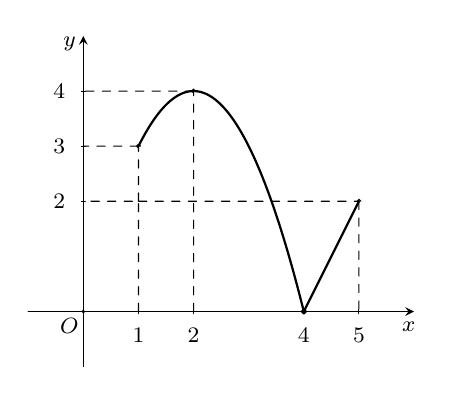
\begin{tikzpicture}[scale=0.7, font=\footnotesize, line join=round,
			line cap=round, >=stealth]
			\def \xmin{-1}
			\def \xmax{6}
			\def \ymin{-1}
			\def \ymax{5}
			\draw[->] (\xmin,0)--(\xmax,0) node[shift=(-110:0.2)] {$x$};
			\draw[->] (0,\ymin)--(0,\ymax) node[shift=(-150:0.2)] {$y$};
			\fill (0,0) circle(1pt) node[shift=(-135:0.25)]{$O$};
			\clip (\xmin,\ymin) rectangle (\xmax,\ymax);
			\draw[smooth,samples=100,domain=1:4,thick] plot(\x,{-(\x)^2+4*(\x)});
			\foreach  \x/\g in {1/-90,2/-90,4/-90,5/-90} 
			\draw (\x,1pt)--(\x,-1pt)+(\g:0.4) node {$\x$};
			\foreach  \y/\g in {2/180,3/180,4/180} 
			\draw (1pt,\y) --(-1pt,\y)+(\g:0.4) node {$\y$};
			\draw[dashed] (1,0)--(1,2)--(0,2) (1,2)--(1,3) circle(1pt)--(0,3) (2,0)--(2,4) circle(1pt)--(0,4) (1,2)--(5,2) circle(1pt)--(5,0);
			\draw[thick] (4,0) circle(1pt)--(5,2);
		\end{tikzpicture}
	\end{center}
	Trên đoạn $[1 ; 5]$, hàm số đã cho đạt giá trị lớn nhất tại điểm
	\choice
	{$x=4$}
	{\True $x=2$}
	{$x=1$}
	{$x=5$}
	\loigiai{Từ đồ thị hàm số, ta có hàm số đã cho đạt giá trị lớn nhất tại điểm $x=2$.}
\end{ex}
\begin{ex}%[2D1H3-1]
	Giá trị nhỏ nhất của hàm số $f(x)=x^3+3x-6$ trên đoạn $[1;3]$ là
	\choice
	{\True $-2$}
	{$-39$}
	{$-6$}
	{$-10$}
	\loigiai{
		Ta có $f'(x)=3x^2+3> 0$ với mọi $x\in\mathbb{R}$.\\
		Hàm số đồng biến trên $[1;3]$ nên giá trị nhỏ nhất của hàm số trên đoạn $[1;3]$ là $f(1)=-2$
	}
\end{ex}
\begin{ex}%[2D1N3-1]
	Cho hàm số $y=f(x)$ liên tục và có bảng biến thiên trên đoạn $[-1;3]$ như hình vẽ bên. Khẳng định nào sau đây đúng?
	\begin{center}
		
\begin{tikzpicture}
			\tkzTabInit[lgt=1.2,espcl=2]
			{$x$ /0.6, $f’(x)$ /0.6, $f(x)$ /1.5}
			{$-1$,$0$,$2$,$3$}
			\tkzTabLine{ ,+,0,-,0,+, }
			\tkzTabVar{-/$0$,+/$5$,-/$1$,+/$4$}
		\end{tikzpicture}
	\end{center}
	\choice
	{$\max\limits_{[-1;3]} f(x)=4$}
	{\True $\max\limits_{[-1;3]} f(x)=5$}
	{$\max\limits_{[-1;3]} f(x)=1$}
	{$\max\limits_{[-1;3]} f(x)=0$} 
	\loigiai{
		Dựa vào bảng biến thiên ta có $\max\limits_{[-1;3]} f(x)=5$.
	}
\end{ex}
\begin{ex}%[2D1H3-1]
	Giá trị nhỏ nhất của hàm số $y=\dfrac{x-2}{x+1}$ trên đoạn $[0;3]$ là
	\choice
	{$\min\limits_{x\in \left[0;3\right]} y=-3$}
	{\True $\min\limits_{x\in \left[0;3\right]} y=-2$}
	{$\min\limits_{x\in \left[0;3\right]} y=\dfrac{1}{4}$}
	{$\min\limits_{x\in \left[0;3\right]} y=-\dfrac{1}{2}$}
	\loigiai{Hàm số $y=\dfrac{x-2}{x+1}$ liên tục trên đoạn $\left[0;3\right]$.\\
		Ta có $y'=\dfrac{3}{(x+1)^2} > 0$ $\forall x\in \left[0;3\right]$.\\
		Vậy $\min\limits_{x\in \left[0;3\right]} y=y(0)=-2$.		
	}
\end{ex}
\begin{ex}%[2D1N3-1]
	\immini {
		Cho hàm số $y=f(x)$ liên tục trên đoạn $[-1;3]$ và có đồ thị như hình vẽ. Gọi $M$, $m$ lần lượt là giá trị lớn nhất và giá trị nhỏ nhất của hàm số $y=f(x)$ trên đoạn $[-1;3]$. Ta có giá trị của $M+2m$ là
		\choice[2]
		{$M+2m=3$}
		{$M+2m=4$}
		{$M+2m=1$}
		{\True $M+2m=2$}
	}{
		\begin{tikzpicture}[scale=0.8,line join=round, line cap=round,>=stealth]
			\def\xmin{-2} \def\xmax{4}
			\def\ymin{-2} \def\ymax{5}
			\draw[->] (\xmin,0)--(\xmax,0) node[below] {$x$};
			\draw[->] (0,\ymin)--(0,\ymax) node[left] {$y$};
			\draw (0,0) node [below left] {$O$};
			\foreach \x/\g in {-1/90,1/-90,3/-90}
			\draw[thin] (\x,1pt)--(\x,-1pt)+(\g:0.4)node[scale=1]{$\x$};
			\foreach \y/\g in {-1/0,1/180,4/180}		
			\draw[thin] (1pt,\y)--(-1pt,\y)+(\g:0.4)node[scale=1]{$\y$};
			\begin{scope}
				\clip (\xmin+0.1,\ymin+0.1) rectangle (\xmax-0.1,\ymax-0.1);
				\draw[thick,red,smooth,samples=300,domain=0:3] plot(\x,{(\x)^2-2*(\x)+1});								
				\draw[thick,red] (-1,-1)--(0,1);
			\end{scope}		
			\foreach \x/\y in {0/0,0/1,-1/-1,3/4}
			\fill[black] (\x,\y) circle(1.2pt);
			\foreach \x/\y in {-1/-1,3/4}
			\draw [dashed, black] (\x,0) |-(0,\y);
			\path (3,4) node[right]{$y=f(x)$}			
			;
		\end{tikzpicture}
	}	
	\loigiai{
		Theo đồ thị trên $[-1;3]$, ta có $M=4$, $m=-1$.\\
		Suy ra $M+2m=4+2\cdot (-1)=2$.\\
	}
\end{ex}

\begin{ex}%[2D1H3-1]
	Giá trị lớn nhất của hàm số $y=x^3-3x+4$ trên đoạn $[-2;0]$ bằng
	\choice
	{$2$}
	{$4$}
	{$12$}
	{\True $6$}
	\loigiai{
		Ta có $y'=3x^2-3$.\\
		Khi đó
		\[y'=0 \Leftrightarrow 3x^2-3=0 \Leftrightarrow
		\hoac{
			&x=1 \notin [-2;0]\\
			&x=-1 \in [-2;0].}\]
		Ta có $y(-2)= 2$; $y(-1)=6$ và $y(0)=4$.\\
		Do đó $\max\limits_{[-2;0]} y=y(-1)=6$.
	}
\end{ex}
\begin{ex}%[2D1H3-2]
	Cho hàm số $y=f(x)$ liên tục trên $\mathbb{R}$ có bảng xét dấu đạo hàm như sau
	\begin{center}
		
\begin{tikzpicture}[>=stealth]
			\tkzTabInit[nocadre=true,lgt=1.2,espcl=2.5,deltacl=0.6]
			{$x$/0.75,$f'(x)$/0.75}
			{$-\infty$, $-1$, $0$, $1$, $+\infty$}
			\tkzTabLine{,-, d,-, 0, +, 0, -,}
		\end{tikzpicture}
	\end{center}
	Mệnh đề nào sau đây đúng?
	\choice
	{\True $\max\limits_{(0;+\infty)} f(x)=f(1)$}
	{$\max\limits_{[-1; 1]} f(x)=f(0)$}
	{$\max\limits_{(-\infty;-1)} f(x)=f(-1)$}
	{$\min\limits_{(0; 1)} f(x)=f(0)$}
	\loigiai{
		Ta có bảng biến thiên của $f(x)$ như sau
		\begin{center}
			
\begin{tikzpicture}[>=stealth]
				\tkzTabInit[nocadre=true,lgt=1.2,espcl=2.5,deltacl=0.6]
				{$x$/0.75,$f'(x)$/0.75,$f(x)$/1.8}
				{$-\infty$, $-1$, $0$, $1$, $+\infty$}
				\tkzTabLine{,-, d,-, 0, +, 0, -,}
				\tkzTabVar{+/, R, -/, +/, -/}
			\end{tikzpicture}
		\end{center}
		Dựa vào bảng biến thiên, ta thấy $\max\limits_{(0;+\infty)} f(x)=f(1)$.
	}
\end{ex}
\Closesolutionfile{ans}
\ind{PHẦN II.} \inden{Câu trắc nghiệm đúng sai. Trong mỗi ý a), b), c), d) ở mỗi câu, học sinh chọn đúng hoặc sai.}\\
\setcounter{ex}{0}
\Opensolutionfile{ans}[ans/2D1-Bai1-DS]
\begin{ex}%[2D1H3-1]
	Cho hàm số $y=f(x)$ liên tục trên $\mathbb{R}$ có bảng xét dấu đạo hàm như sau:
	\begin{center}
		
\begin{tikzpicture}
			\tkzTabInit[nocadre=true,lgt=1.2,espcl=3, deltacl=0.5]
			{$x$ /0.7,$f’(x)$ /0.7}
			{$-\infty$,$1$,$3$,$+\infty$}
			\tkzTabLine{,+,0,-,0,+,}
		\end{tikzpicture}
	\end{center}
	\choiceTF
	{\True Hàm số $y=f(x)$ đồng biến trên $(-\infty;1)$ và $(3;+\infty)$}
	{\True Điểm cực tiểu của hàm số bằng $3$} 
	{Hàm số $y=f(x)$ có $2$ điểm cực trị trái dấu}
	{Giá trị nhỏ nhất của hàm số $h(x)=f'(x)$ trên $[1;3]$ là $2$ biết $f'(x)=3x^2+bx+c$}
	\loigiai{
		\begin{itemchoice}
			\itemch  Dựa vào bảng xét dấu, hàm số $y=f(x)$ đồng biến trên $(-\infty;1)$ và $(3;+\infty)$.
			\itemch  Dựa vào bảng xét dấu, điểm cực tiểu của hàm số bằng $3$.
			\itemch  Hàm số có $2$ điểm cực trị cùng dấu là $x=1$ và $x=3$.
			\itemch  $f'(x)=0$ có hai nghiệm là $x=1$; $x=3$. \\
			Suy ra
			\[\heva{&3\cdot 1+b+c=0 \\&3\cdot 3^2+3 b+c=0 } \Rightarrow \heva{&b=-12 \\&c=9} \Rightarrow f'(x)=3 x^2-12x+9.\]
			Xét hàm số $g(x)=3x^2-12x+9$.\\
			Ta có $g'(x)=6x-12$.\\
			Khi đó 
			\[g'(x)=0 \Leftrightarrow x=2.\]
			Ta có $g(1)=0$, $g(2)=-3$ và $g(3)=0$.\\
			Vậy $\min\limits_{[1;3]} f'(x)=\min\limits_{[1;3]} g(x)=g(2)=-3$.
			
		\end{itemchoice}	
	}
\end{ex}

\begin{ex}%[2D1H3-1]
	Cho hàm số $f(x)=x-\sin 2 x$.
	\choiceTF
	{\True $f(0)=0 ; f(\pi)=\pi$}
	{Đạo hàm của hàm số đã cho là $f'(x)=1+2 \cos 2 x$}
	{\True Nghiệm của phương trình $f'(x)=0$ trên đoạn $[0 ; \pi]$ là $\dfrac{\pi}{6}$ và $\dfrac{5 \pi}{6}$}
	{\True Giá trị nhỏ nhất của hàm số đã cho trên đoạn $[0 ; \pi]$ là $\dfrac{\pi}{6}-\dfrac{\sqrt{3}}{2}$}
	\loigiai{
		\begin{itemchoice}
			\itemch Ta có
			$f(0)=0-\sin 2 .0=0$ và $f(\pi)=\pi-\sin 2 \pi=\pi$.
			\itemch Ta có  $f'(x)=1-2 \cos 2 x$.
			\itemch 
			Ta có 
			\[f'(x)=0 \Leftrightarrow \cos 2x=\dfrac{1}{2} \Leftrightarrow \hoac{&x=\dfrac{\pi}{6} +k2\pi\\&x=-\dfrac{\pi}{6}+k2\pi} (k \in \mathbb{Z}). \]
			Với $x \in [0;\pi]$, ta có $x=\dfrac{\pi}{6}$ và $x=\dfrac{5\pi}{6}$.\\
			Suy ra $x=\dfrac{\pi}{6}$ và $x=\dfrac{5 \pi}{6}$ là nghiệm của phương trình $f'(x)=0$ trên đoạn $[0 ; \pi]$.
			
			\itemch 
			Ta có $f(x)=x-\sin 2 x, f'(x)=1-2 \cos 2 x$ có nghiệm $x=\dfrac{\pi}{6}$, $\dfrac{5 \pi}{6}\in[0 ; \pi]$.\\
			Ta có $f(0)=0$; $f(\pi)=\pi$; $f\left(\dfrac{\pi}{6}\right)=\dfrac{\pi}{6}-\dfrac{\sqrt{3}}{2}$; $f\left(\dfrac{5 \pi}{6}\right)=\dfrac{5 \pi}{6}+\dfrac{\sqrt{3}}{2}$. \\
			Do đó, giá trị nhỏ nhất của $f(x)$ trên đoạn $[0 ; \pi]$ là $\dfrac{\pi}{6}-\dfrac{\sqrt{3}}{2}$.
		\end{itemchoice}
	}
\end{ex}
\begin{ex}%[2D1H3-6]
	Một vật chuyển động theo quy luật $s(t)=t^3-3t^2+9t+36$, với $t$ (giây) là khoảng thời gian tính từ lúc chất điểm bắt đầu chuyển động và $s$ là quãng đường vật đi được trong khoảng thời gian đó, tính bằng mét.  
	\choiceTF
	{Quãng đường vật đi được sau $4$ giây kể từ lúc bắt đầu chuyển động là $82$ m}
	{\True Vận tốc của vật tại giây thứ $t$ là $v(t)=3t^2-6t+9$}
	{Gia tốc của vật tại thời điểm $2$ giây là $4$ m/s$^2$}
	{\True Trong khoảng thời gian $10$ (s) đầu tiên, vận tốc của vật nhỏ nhất là $6$ m/s}
	\loigiai{
		\begin{itemchoice}
			\itemch Quãng đường vật đi được sau $4$ giây kể từ lúc bắt đầu chuyển động là
			$$
			s(4)=4^3-3 \cdot 4^2+9 \cdot 4+36=88 \, \text{m}.
			$$
			\itemch 
			Vận tốc của vật tại giây thứ $t$ là
			$$
			v(t)=s'(t)=3t^2-6t+9.
			$$			
			\itemch 
			Gia tốc của vật tại giây thứ $t$ là
			$$
			a(t)=v'(t)= 6t-6.
			$$
			Khi đó
			$$
			a(2)=6 \cdot 2-6=12-6=6 \, \text{m/s}^2.
			$$
			\itemch
			Ta có
			\[v'(t)=6t-6.\]
			Khi đó
			\[v'(t)=0\Leftrightarrow 	6t-6=0  \Leftrightarrow  t=1.\]
			Bảng biến thiên 
			\begin{center}
				
\begin{tikzpicture}
					\tkzTabInit[lgt=1.5,espcl=2]
					{$t$/1, $v'(t)$/1, $v(t)$/2}
					{$0$, $1$, $10$}
					\tkzTabLine{,-,0,+,}
					\tkzTabVar{+/ $9$, -/ $6$, +/ $249$}
				\end{tikzpicture}
			\end{center}	
			Giá trị nhỏ nhất của $v(t)$ trên $[0; 10]$ là $v(1)=6$ m/s.
		\end{itemchoice}
	}
\end{ex}
\begin{ex}%[2D1H3-6]
	Mỗi đợt xuất khẩu gạo của tỉnh $A$ kéo dài trong $60$ ngày. Người ta thấy sản lượng gạo xuất khẩu theo ngày thứ $t$ được xác định bởi công thức $s(t)=-t^3+27t^2+262\,144$ (tấn) với $1\le t\le 60$, $t\in\mathbb{N^{*}}$.
	\choiceTF
	{\True Sản lượng gạo xuất khẩu của tỉnh $A$ ngày thứ $12$ là $264\,304$ (tấn)}
	{Ngày thứ $30$ tỉnh $A$ có sản lượng gạo xuất khẩu cao nhất}
	{Ngày thứ $1$ tỉnh $A$ có sản lượng gạo xuất khẩu thấp nhất}
	{\True Ngày thứ $60$ tỉnh $A$ có sản lượng gạo xuất khẩu thấp nhất là $143\,344$ (tấn)}
	\loigiai
	{
		\begin{itemchoice}
			\itemch Ta có $s(12)=-(12)^3+27\cdot(12)^2+262\,144=264\,304$ (tấn).
			\itemch Ta có $s'(t)=-3t^2+54t$, $s'(t)=0 \Leftrightarrow -3t^2+54t=0 \Leftrightarrow \hoac{&t=0 \\ & t=18.}$ \\
			Bảng biến thiên
			\begin{center}
				
\begin{tikzpicture}[scale=1]
					\tkzTabInit[nocadre=false, lgt=1.2, espcl=2.5, deltacl=0.6]{$x$/0.6, $s'(t)$/0.6, $s(t)$/2}{$1$, $18$, $60$}
					\tkzTabLine{,+,0,-,}
					\tkzTabVar{-/$262\,170$, +/$265\,060$, -/$143\,344$ }
				\end{tikzpicture}
			\end{center}
			Vậy ngày thứ $18$ tỉnh $A$ có lượng gạo xuất khẩu cao nhất là $265\,060$ (tấn).
			\itemch Ngày thứ $1$ tỉnh $A$ có sản lượng xuất khẩu gạo là $262\,170$ nhiều hơn ngày thứ $60$ (tấn).
			\itemch Ngày thứ $60$ của tỉnh $A$ có sản lượng xuất khẩu gạo thấp nhất là $143\,344$.
		\end{itemchoice}
	}
\end{ex}
\begin{ex}%[2D1H3-6]
	\immini[thm]
	{Một chiếc đèn được đặt trên đỉnh của một cột đèn cao $h$ (m) để chiếu sáng một vòng xuyến giao thông đông đúc có bán kính $12$ m. Cường độ ánh sáng $I$ tại một điểm $P$ trên vòng xuyến tỉ lệ thuận với cosin của góc $\theta$ và tỉ lệ nghịch với bình phương khoảng cách $d$ (m) từ nguồn sáng đến điểm $P$.
	}{\begin{tikzpicture}[>=stealth,line join=round,line cap=round,scale=0.5]
			\path (0,0)coordinate(O) (-0.2,0)coordinate(A) (0.2,0)coordinate(B) (0.2,0.5)coordinate(C) (-0.2,0.5)coordinate(D) (-0.1,0.5)coordinate(E) (0.1,0.5)coordinate(F) (0.1,7)coordinate(G) (-0.1,7)coordinate(H) (-0.4,7.8)coordinate(I) (0.4,7.8)coordinate(J) (0.2,8.2)coordinate(K) (-0.2,8.2)coordinate(L) (5,0)coordinate[label=right:$P$](P);
			\coordinate (M) at ($(G)!0.5!(H)$);
			\coordinate (N) at ($(E)!0.5!(F)$);
			\coordinate (Q) at ($(K)!0.5!(L)$);
			\coordinate (S) at ($(Q)+(0,0.1)$);
			\fill[black] (P)circle(1pt);
			\fill[color=black] (A)--(B)--(C)--(D)--(A)  (E)--(F)--(G)--(H)--(E)  (I)--(J)--(K)--(L)--(I);
			\draw[thick] (I)--(H)--(G)--(J);
			\draw[black] (O) ellipse (5cm and 2cm);
			\draw[dashed] (O) ellipse (4.5cm and 1.4cm);
			\draw[black] (O) ellipse (3.5cm and 1cm);
			\draw[black,fill=black] (S) circle (0.1cm);
			\draw (O) -- node[midway, below] {$12$ m} (P);
			\draw (M) -- node[midway, above] {$d$} (P);
			\draw (E) -- node[midway, left] {$h$} (G);
			\path pic[angle radius=6mm,draw=blue,"$\theta$",angle eccentricity=1.5] {angle=N--M--P};
	\end{tikzpicture}}
	\choiceTF
	{\True $I=k \dfrac{\cos \theta}{d^2}$ (với $k$ là hằng số dương)}
	{$\cos \theta=\dfrac{12}{\sqrt{h^2+144}}$}
	{Nếu $I=f(h)$ thì $f'(h)=k \dfrac{-2h^2+144}{\left(h^2+144\right)^2 \sqrt{\left(h^2+144\right)^3}}$}
	{\True Để cường độ ánh sáng $I$ lớn nhất thì cột đèn phải cao $6\sqrt{2}$ m}
	\loigiai{
		\begin{itemchoice}
			
			\itemch
			Theo giả thiết $I=k \dfrac{\cos\theta}{d^2}$ (với $k$ là hằng số dương).
			\itemch
			Ta có $\cos\theta=\dfrac{h}{d}=\dfrac{h}{\sqrt{h^2+144}} \neq \dfrac{12}{\sqrt{h^2+144}}$.
			\itemch
			Ta có $I=k \dfrac{\cos\theta}{d^2}=k \dfrac{h}{\sqrt{h^2+144}} \cdot \dfrac{1}{h^2+144}=k \dfrac{h}{\sqrt{(h^2+144)^3}}$.\\
			Khi đó 
			\begin{eqnarray*}
				f'(h) &=&k \dfrac{\sqrt{(h^2+144)^3}-h \cdot \dfrac{3}{2}\cdot\sqrt{h^2+144}\cdot 2h}{(h^2+144)^3}\\ &=& k \dfrac{\sqrt{h^2+144}\cdot \left(h^2+144-3h^2\right)}{(h^2+144)^3}\\&=&k \dfrac{- 2h^2+144}{(h^2+144)^2\cdot \sqrt{h^2+144}}.
			\end{eqnarray*}
			\itemch
			Xét $f'(h)=0 \Leftrightarrow 144-2h^2=0 \Leftrightarrow h=6\sqrt{2}$.\\
			Bảng biến thiên
			\begin{center}
				
\begin{tikzpicture}[>=stealth]
					\tkzTabInit[nocadre=false,lgt=1.2,espcl=2,deltacl=0.5]{$x$/.7 ,$f'(h)$/.7,$f(h)$/2}
					{$0$ , $6\sqrt{2}$ , $+\infty$}
					\tkzTabLine{ ,+, $0$ ,-, }
					\tkzTabVar{-/$ $ , +/$ $ , -/$ $}
				\end{tikzpicture}
			\end{center}
			Vậy để cường độ ánh sáng $I$ lớn nhất thì cột đèn phải cao $6\sqrt{2}$ m.
		\end{itemchoice}
	}
\end{ex}
\Closesolutionfile{ans}
\ind{PHẦN III.} \inden{Câu trắc nghiệm trả lời ngắn. Học sinh điền đáp án vào ô bên dưới}\\
\setcounter{ex}{0}
\Opensolutionfile{ans}[ans/2D1-Bai1-DS]
\begin{ex}
	Một bờ hồ hình bán nguyệt có bán kính bằng $2$ km, đường kính là đoạn $AB$. Từ điểm $A$, anh Việt chèo một chiếc thuyền với vận tốc $3$ km/h đến điểm $C$ trên bờ hồ (khác $A$ và $B$), rồi chạy bộ dọc theo bờ hồ từ $C$ đến $B$ với vận tốc $6$ km/h, như hình vẽ minh họa dưới đây.
	\begin{center}
		\begin{tikzpicture}[scale=0.7, font=\footnotesize, line join=round,line cap=round, >=stealth]
			\path
			(-4,0) coordinate (A)
			(0,0)+(60:4) coordinate (C)
			(4,0) coordinate (B)
			(0,0) coordinate (O)
			;
			\draw[pattern=north east lines] (-4,0)--(4,0)--(4,-0.25)--(-4,-0.25)--cycle;
			\draw (4,0) arc (0:180:4);
			\draw[->,thick] (A)--(C);
			\draw[->,thick,dashed] (C)--(B);
			\foreach \i/\g in {A/180,B/0,C/90,O/90} \fill (\i) circle(1.5pt)+(\g:0.5) node{$\i$};
		\end{tikzpicture}
	\end{center}
	Biết rằng đoạn đường từ $A$ đến $C$ là đoạn đường thẳng qua mặt hồ và đoạn từ $C$ đến $B$ là một phần của đường cong bán nguyệt.
	Hỏi thời gian lớn nhất mà anh Việt di chuyển từ $A$ đến $B$ là bao nhiêu? (Thời gian tính bằng giờ, kết quả làm tròn đến hàng phần chục).
	\par \shortans{1,5}
	\loigiai{
		\begin{center}
			\begin{tikzpicture}[scale=0.7, font=\footnotesize, line join=round,line cap=round, >=stealth]
				\path
				(-4,0) coordinate (A)
				(0,0)+(60:4) coordinate (C)
				(4,0) coordinate (B)
				(0,0) coordinate (O)
				;
				\draw[pattern=north east lines] (-4,0)--(4,0)--(4,-0.25)--(-4,-0.25)--cycle;
				\draw (4,0) arc (0:180:4);
				\draw[->,thick] (A)--(C);
				\draw[->,thick,dashed] (C)--(B);
				\foreach \i/\g in {A/180,B/0,C/90,O/90} \fill (\i) circle(1.5pt)+(\g:0.5) node{$\i$};
				\draw pic["$\alpha$",draw,angle eccentricity=1.5,angle radius=0.5cm]{angle=B--A--C};
				\draw pic[draw,angle radius=0.3cm]{right angle=A--C--B};
			\end{tikzpicture}
		\end{center}
		Đặt $\widehat{BAC}=\alpha$ với $\left(0<\alpha<\dfrac{\pi}{2}\right)$.\\
		Vì $\widehat{ACB}$ là  góc nội tiếp chắn nửa đường tròn nên $\widehat{ACB}=90^\circ$.\\
		$\triangle ABC$ vuông tại $C$ nên $AC=AB \cdot \cos \alpha=4\cos \alpha$.\\
		Lại có $\widehat{BAC}$ là góc nội tiếp chắn cung $BC$ nên $\widehat{BAC}=\dfrac{1}{2}$ sđ$\wideparen{BC}$ hay sđ$\wideparen{BC}=2\alpha$.\\
		Khi đó ta có $l_{\wideparen{BC}}=2 \cdot 2\alpha=4\alpha$.\\
		Suy ra tổng thời gian anh Việt đã đi là
		\[t=\dfrac{4\cos\alpha}{3}+\dfrac{4\alpha}{6}=\dfrac{4}{3} \cos \alpha+\dfrac{2}{3} \alpha \ (\text{h}).\]
	Xét hàm số $f(\alpha)=\dfrac{4}{3} \cos \alpha+\dfrac{2}{3} \alpha$ với $0<\alpha<\dfrac{\pi}{2}$.\\
	Ta có
	\[f'(\alpha)=-\dfrac{4}{3} \sin \alpha+\dfrac{2}{3}.\]
	Khi đó
	\[f'(\alpha)=0 \Leftrightarrow \sin \alpha=\dfrac{1}{2} \Leftrightarrow \alpha= \dfrac{\pi}{6}.\]
	Bảng biến thiên
	\begin{center}
		
\begin{tikzpicture}[scale=1, font=\footnotesize, line join=round, line cap=round, >=stealth]
			\tkzTabInit[nocadre=true,lgt=1.2,espcl=2.5,deltacl=0.6]
			{$\alpha$ /1, $f'(\alpha)$ /1, $f(\alpha)$ /2} 
			{$0$,$\dfrac{\pi}{6}$, $\dfrac{\pi}{2}$}
			\tkzTabLine{,+,0,-,}
			\tkzTabVar{-/ , +/$\dfrac{2\sqrt{3}}{3}+\dfrac{\pi}{9}$ ,-/}
		\end{tikzpicture}
	\end{center}
	Vậy thời gian lớn nhất mà anh Việt di chuyển từ $A$ đến $B$ là $1{,}5$ giờ.
}
\end{ex}
\begin{ex}%[2D1V3-3]
	(\textit{Đề thi HK1 Trường THPT Marie Curie -- HCM -- Năm 2024 -- 2025}) \\
	Một con đường cần được xây dựng giữa hai thành phố $X$ và $Y$ nằm ở hai bên đối diện của một con sông có chiều rộng đều  bằng $1$ km. Thành phố $X$ cách sông $2$ km và $Y$ cách sông $4$ km, khoảng cách giữa hai hình chiếu vuông góc của $X$ và $Y$ trên bờ sông là $X'Y'=6$ km. Một cây cầu sẽ được xây dưng để cho phép giao thông đi qua sông. Vị trí của cây cầu $CD$ cách $XX'$ là $x$ (km). Tìm $x$ để con đường cần được xây dựng giữa hai thành phố $X$ và $Y$ được ngắn nhất.
	\begin{center}
		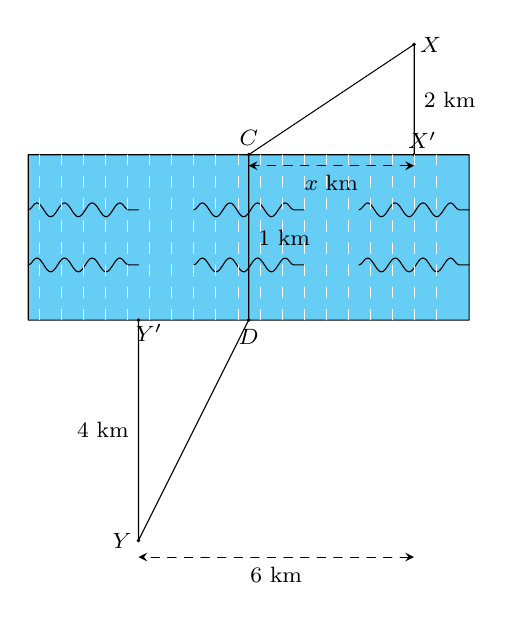
\begin{tikzpicture}[scale=0.7, font=\footnotesize,line join=round, line cap=round, >=stealth]
			\def\a{8} %%chiều dài
			\def\b{3} %%chiều rộng
			\path 
			(0,0) coordinate (A)
			(\a,0) coordinate (B)
			(8,3) coordinate (K)
			(7,5) coordinate (X)
			(7,3) coordinate (X')
			(2,-4) coordinate (Y)
			(2,0) coordinate (Y')
			(4,0) coordinate (D)
			(4,3) coordinate (C)
			;
			\draw [fill=cyan!60](A)--(B)--(K)--(0,3)--(A);
			\draw (X')--(X)--(C)--(D)--(Y)--(Y');
			\draw (X)--(X')node[right,midway]{$2$ km};
			\draw (Y)--(Y')node[left,midway]{$4$ km};
			\draw (D)--(C)node[right,midway]{$1$ km};
			\draw[dashed,<->] (7,-4.3)--(2,-4.3)node[midway,below]{$6$ km};
			\draw[dashed,<->] (7,2.8)--(4,2.8)node[midway,below]{$x$ km};
			\foreach \i/\g in {C/90,D/-90,X/0,Y/180,X'/60,Y'/-50}
			\fill[black] (\i) circle(1pt)+(\g:3mm)node[scale=1]{$\i$};
			\draw[decorate,decoration=snake] (0,1)-- (2,1) ;
			\draw[decorate,decoration=snake] (0,2)-- (2,2) ;
			\draw[decorate,decoration=snake] (3,1)-- (5,1) ;
			\draw[decorate,decoration=snake] (3,2)-- (5,2) ;
			\draw[decorate,decoration=snake] (6,1)-- (8,1) ;
			\draw[decorate,decoration=snake] (6,2)-- (8,2) ;
			\foreach \i in {0.2,0.6,...,7.8}
			\draw[ultra thin,white,dash pattern=on 4pt off 4pt] (\i,0)--(\i,3);
		\end{tikzpicture}
		\par	\shortans{2}
	\end{center}	
	\loigiai{Theo giả thiết ta có $XX'=2$, $YY'=4$, $CD=1$.\\
		Ta tính được $CX=\sqrt{x^2+4}$, $DY=\sqrt{4^2+(6-x)^2}$.\\
		Quãng đường hai thành phố có độ dài là 
		\[f(x)=XC+CD+DY=1+\sqrt{x^2+4}+\sqrt{x^2-12x+52}.\]
		Xét hàm số $f(x)=1+\sqrt{x^2+4}+\sqrt{x^2-12x+52}$ với $0<x<6$.\\
		Ta có $f'(x)=\dfrac{x}{\sqrt{x^2+4}}+\dfrac{x-6}{x^2-12x+52}$. \\
		Khi đó
		\begin{eqnarray*}
			f'(x)=0 & \Leftrightarrow& \dfrac{x}{\sqrt{x^2+4}}=\dfrac{6-x}{\sqrt{x^2-12 x+52}} \\
			& \Leftrightarrow& \dfrac{x^2}{x^2+4}=\dfrac{(6-x)^2}{x^2-12 x+52}, \quad(0<x<6) \\
			& \Leftrightarrow& \dfrac{x^2}{x^2+4}-1=\dfrac{x^2-12 x+36}{x^2-12 x+52}-1 \\
			& \Leftrightarrow&-\dfrac{4}{x^2+4}=-\dfrac{16}{x^2-12 x+52} \\
			& \Leftrightarrow& x^2-12 x+52=4\left(x^2+4\right) \\
			& \Leftrightarrow & 3 x^2+12 x-36=0 \\
			& \Leftrightarrow&\hoac{&x=2\\&x=-6\text{ (Loại).}}
		\end{eqnarray*}
		Bảng biến thiên
		\begin{center}
			
\begin{tikzpicture}[>=stealth]
				\tkzTabInit[nocadre=true,lgt=1.2,espcl=2.5,deltacl=0.6]
				{$x$ /1, $f'(x)$ /1, $f(x)$ /2} 
				{$0$,$2$,$6$}
				\tkzTabLine{,-,0,+,}
				\tkzTabVar{+/ , -/ $6\sqrt{2}+1$ , +/}
			\end{tikzpicture}
		\end{center}
		Để con đường cần được xây dựng giữa hai thành phố $X$ và $Y$ được ngắn nhất thì $x=2$.}
\end{ex}
\begin{ex}%[Text ĐTT các trường Sở, KHTN Hà Nội 2025, Huỳnh Xuân Tín]%[2D1V3-6]
	(\textit{Đề thi thử -- Trường chuyên KHTN -- Hà Nội -- năm 2024 -- 2025})\\
	Giả sử chi phí đặt hàng và vận chuyển $C$ (đơn vị: triệu đồng) của một linh kiện được sử dụng trong sản xuất một sản phẩm được xác định theo công thức $C=\dfrac{19\,200\,000}{x^2}+\dfrac{27x}{x+3\,000}$, $x \geq 1$. Trong đó $x$ là số linh kiện được đặt hàng và vận chuyển. Tìm $x$ để chi phí đặt hàng và vận chuyển cho mỗi linh kiện trên là nhỏ nhất.
	\shortans{2400}
	\loigiai{
		Xét hàm số $C(x)=\dfrac{19\,200\,000}{x^2}+\dfrac{27x}{x+3\,000}$, $x \geq 1$.\\
		Ta có $C'(x)=-\dfrac{38\,400\,000}{x^3}+\dfrac{81\,000}{(x+3\,000)^2}$.
		$$\begin{aligned}
			C'(x)=0 & \Leftrightarrow \dfrac{38\,400\,000}{x^3}=\dfrac{81\,000}{(x+3\,000)^2} \\
			& \Leftrightarrow 12\,800(x+3\,000)^2=27 x^3 \Leftrightarrow x=2\,400.
		\end{aligned}$$	
		Ta có bảng biến thiên
		\begin{center}
			
\begin{tikzpicture}
				\tkzTabInit[nocadre=false,lgt=1.2,espcl=2.5,deltacl=0.6]
				{$x$/.6 ,$f'(x)$/.6,$f(x)$/2.5}
				{$1$ ,$2\,400$, $+\infty$}
				\tkzTabLine{ ,-, $0$ ,+, }
				\tkzTabVar{+/,-/, +/}
			\end{tikzpicture}
		\end{center}		
		Vậy chi phí đặt hàng và vận chuyển cho mỗi linh kiện trên là nhỏ nhất khi $x=2\,400$.}
\end{ex}
\begin{ex}%[2D1V3-6]
	(\textit{Đề thi HK1 THPT Ngô Quyền-TPHCM năm 2023 -- 2024})\\
	Ông Nam cần xây dựng một bể chứa nước có dạng hình hộp chữ nhật không có nắp đậy để phục vụ cho việc tưới cây trong vườn. Do các điều kiện về diện tích vườn, ông Nam cần bể có thể tích là $36$ mét khối, đáy bể có chiều dài gấp hai lần chiều rộng và chiều rộng không quá $4$ mét, biết rằng chi phí vật liệu xây dựng mỗi mét vuông diện tích bề mặt là như nhau. Hỏi chiều cao bể nước bằng bao nhiêu mét để tổng chi phí vật liệu là nhỏ nhất?
	\par \shortans{$2$}
	\loigiai{Gọi chiều rộng của đáy bể là $x$ (mét) với $0<x\le 4$.\\
		Chiều dài của đáy bể là $2x$.\\
		Gọi $h$ (mét) là chiều cao của bể.\\
		Thể tích của bể là $V=h\cdot x \cdot 2x=2hx^2$.
		Suy ra $h=\dfrac{36}{2x^2}=\dfrac{18}{x^2}$. \qquad (1)\\
		Gọi $S$ là diện tích bề mặt của bể (không tính nắp).\\
		$S$ là tổng diện tích đáy và diện tích bốn mặt bên.\\
		Do đó $S=2x^2+2\cdot x\cdot h+2\cdot 2x\cdot h=2x^2+6hx$. \qquad (2)\\
		Từ (1) và (2) suy ra $S=2x^2+6x\cdot \dfrac{18}{x^2}=2x^2+\dfrac{108}{x}$.\\
		Xét hàm số $f(x)=2x^2+\dfrac{108}{x}$ với $0<x\le 4$.\\
		Ta có $f'(x)=4x-\dfrac{108}{x^2}$.\\
		Khi đó 
		\[f'(x)=0\Leftrightarrow 4x-\dfrac{108}{x^2}=0 \Leftrightarrow x=3.\]
		Bảng biến thiên
		\begin{center}
			
\begin{tikzpicture}
				\tkzTabInit[lgt=1.2,espcl=2.5,deltacl=0.7]
				{$x$ /0.7,$f(x)’$ /0.6,$f(x)$ /2}
				{$+\infty$,$3$,$+\infty$}
				\tkzTabLine{,-,0,+,}
				\tkzTabVar{+/,-/$f(3)$,+/}
			\end{tikzpicture}
		\end{center}
		Từ bảng biến thiên ta có 
		$\min\limits_{x\in (0;4]}f(x)=f(3)=54$ khi $x=3$.\\ Suy ra chiều cao của bể khi đó là $h=\dfrac{18}{3^2}=2$.\\
		Vậy để chi phí vật liệu là nhỏ nhất thì chiều cao của bể là $2$  (m).}
\end{ex}
\begin{ex}%[2D1C3-6]
	(\textit{Đề thi trường THPT Trúc Ninh -- Nam Định -- Lần 1 -- Năm 2024 -- 2025})
	\immini{
		Một hòn đảo nằm trong một hồ nước. Biết rằng đường cong tạo nên hòn đảo được mô hình hóa vào hệ trục tọa độ $Oxy$ là một phần của đồ thị hàm số bậc ba $y=f(x)$. Vị trí điểm cực đại là $(2;5)$ với đơn vị của hệ trục là $100$ m và vị trí điểm cực tiểu là $(0;1)$. Mặt đường chạy trên một đường thẳng có phương trình $y=36-9x$. Người ta muốn làm một cái cây cầu có dạng một đoạn thẳng nối từ hòn đảo ra mặt đường. Độ dài ngắn nhất của cây cầu bằng bao nhiêu mét? (làm tròn đến hàng phần chục)
	}{
		\begin{tikzpicture}[line join=round, line cap=round, >=stealth, font=\footnotesize, scale=0.8]
			\draw[-stealth](0,0)--(0,0)node[above left]{$O$}--(6,0)node[below]{\color{blue}$x$};
			\draw[-stealth](0,0)--(0,6)node[left]{\color{blue}$y$};
			\clip(0,0)rectangle(7,6);
			\tikzset{label style/.style={font=\footnotesize}}
			\draw[cyan,dashed] (-1,-1) grid (6,6);
			%			\draw[->] (-1,0)--(0,0) node[above right]{$O$} -- (6,0) node[above]{$x$};
			%			\draw[->] (0.,-1) -- (0.,6) node[right]{$y$};
			\draw plot[smooth,tension=0.9] coordinates{(-0.5,2) (0.2,1.2) (2,5) (3.1,-0.2)};
			\draw (3,0) node[above right]{$f(x)$};
			\draw (2,2) node{Hòn đảo};
			\draw (3.2,6)--(4.2,-0.6);
			\draw (4,5) node[right]{Mặt đường};
			\draw (5,3) node{$y=36-9x$};
		\end{tikzpicture}
	}
	\shortans{$88{,}3$}
	\loigiai{
		Gọi hàm số bậc ba có dạng $f(x)=ax^3+bx^2+cx+d$. Khi đó $f'(x)=3ax^2+2bx+c$.\\
		Đồ thị hàm số đi qua hai điểm $(0;1)$ và $(2;5)$ nên ta có $d=1$ và $8a+4b+2c+d=5$. \\
		Vì hàm số có hai điểm cực trị $x=0$ và $x=2$ nên $f'(0)=f'(2)=0$, suy ra $c=0$ và $12a+4b=0$. \\
		Từ các phương trình trên ta suy ra $a=-1$, $b=3$, $c=0$, $d=1$. \\
		Suy ra $f(x)=-x^3+3x^2+1$ và $f'(x)=-3x^2+6x$.\\
		Gọi $M(x_0;y_0)$, $x_0>0$ là điểm nằm trên hòn đảo và nối với mặt đường và $d$ là tiếp tuyến của đồ thị hàm số song song với mặt đường. Suy ra $M$ là tiếp điểm của $d$ với $y=f(x)$. \\
		Đường thẳng $y=36-9x$ có hệ số góc $k=-9$ nên
		$$f'(x_0)=-9\Leftrightarrow -3x_0^2+6x_0=-9\Leftrightarrow \hoac{&x_0=3\\&x_0=-1}\Rightarrow x_0=3\Rightarrow M(3;1).$$
		Độ dài cây cầu ngắn nhất bằng khoảng cách từ điểm $M$ đến đường thẳng $9x+y-36=0$ và bằng $\dfrac{4\sqrt{82}}{41}\approx 0{,}883$.\\
		Vì đơn vị của hệ trục là $100$ m nên độ dài ngắn nhất của cây cầu là $88{,}3$ m.
	}
\end{ex}
\Closesolutionfile{ans}
\ind{PHẦN IV.} \inden{Tự luận.}\\
\setcounter{ex}{0}
\begin{ex}%[2D1V3-6]
	(\textit{Đề kiểm tra HK1 -- Trường THPT Mạc Đĩnh Chi -- Năm 2024--2025})\\
	Một vật chuyển động thẳng được xác định bởi phương trình $s(t)=-\dfrac{1}{6} t^3+4 t^2$ với $t$ là khoảng thời gian tính bằng giây từ lúc vật bắt đầu chuyển động và $s$ tính bằng mét là quãng đường vật đi được trong khoảng thời gian $t$ đó. Hỏi trong khoảng thời gian $16$ giây kể từ lúc vật bắt đầu chuyển động, vận tốc của vật đạt giá trị lớn nhất bằng bao nhiêu m/s?
	\loigiai{
		Ta có $v(t)=s'(t)= -\dfrac{1}{2}t^2+8t$.\\
		Vậy ta sẽ tìm giá trị lớn nhất của $v(t)$ trên đoạn $[0;16]$.\\
		Khi đó $v'(t)=-t+8$. Cho $v'(t)=0 \Leftrightarrow t=8$.\\
		Ta có $v(0)=0$, $v(8)= 32$, $v(16)=0$.\\
		Do đó giá trị lớn nhất của $v(t)$ là $32$ (m/s) khi $t=8$ (giây).
	}
\end{ex}
\begin{ex}%[2D1H3-6]
	(\textit{Đề thi thử -- Sở Phú Thọ -- Năm 2024--2025})\\
	Một doanh nghiệp sản xuất độc quyền một loại sản phẩm. Giả sử khi sản xuất và bán hết $x$ sản phẩm $(0<x \leq 2\,500)$, tổng số tiền doanh nghiệp thu được là $f(x)=2\,006 x-x^2$ và tổng chi phí là $g(x)=x^2+1\,438 x-1\,209$ (đơn vị: nghìn đồng). Giả sử mức thuế phụ thu trên một đơn vị sản phẩm bán được là $t$ (nghìn đồng) $(0<t<320)$. Giá trị của $t$ bằng bao nhiêu nghìn đồng để nhà nước nhận được số tiền thuế phụ thu lớn nhất và doanh nghiệp cũng nhận được lợi nhuận lớn nhất theo mức thuế phụ thu đó?
	\loigiai{
		Ta có hàm lợi nhuận:
		\begin{eqnarray*}
			P(x)&=&f(x)-g(x)-x t\\
			&=&2\,006 x-x^2-\left(x^2+1\,438 x-1\,209\right)-x t \\
			& =&-2 x^2+568 x-x t+1\,209 \\
			& =&-2 x^2+(568-t) x+1\,209.
		\end{eqnarray*}
		Khi lợi nhuận lớn nhất $P(x)$ thì $x=\dfrac{-b}{2 a}=-\dfrac{568-t}{2(-2)}=\dfrac{568-t}{4}$.\\
		Khi đó, số tiền thuế thu được $x t=\dfrac{568-t}{4} \cdot t=\dfrac{1}{4}t \cdot(568-t) \leq \dfrac{1}{4}\left(\dfrac{568-t+t}{2}\right)^2=20\,164$.\\
		Dấu \lq\lq$=$\rq\rq \, xảy ra khi $568-t=t \Leftrightarrow t=284 \in(0 ; 320)$ (Thỏa mãn).
	}
\end{ex}
\begin{ex}%[2D1V3-6]
	(\textit{Đề kiểm tra HK1 -- Trường THPT Phụ Dực -- Năm 2024--2025})
	\immini{
		Thầy Nam muốn làm một bể cá cảnh dạng hình hộp chữ nhật không nắp (tham khảo hình minh họa). Biết mặt đáy của bể là hình chữ nhật có kích thước chiều dài gấp $2$ lần chiều rộng, thể tích của bể là $1$ m$^3$. Chi phí làm mỗi m$^2$ mặt đáy là $1$ triệu đồng và chi phí làm mỗi m$^2$ phần xung quanh của bể là $400$ nghìn đồng. Thầy Nam đã thiết kế kích thước của bể tối ưu giúp chi phí làm bể là ít nhất. Trên cơ sở đó thầy dự tính số tiền làm bể là $a$ triệu đồng. Số $a$ là bao nhiêu? (\textit{làm tròn kết quả đến hàng phần trăm})
	}{
		\begin{tikzpicture}[>=stealth,line join=round,line cap=round,font=\footnotesize,scale=1]
			\path 
			(0,0) coordinate (A)
			(0.7,-1.4) coordinate (B)
			(6,-1.4) coordinate (C)
			($(A)-(B)+(C)$) coordinate (D)
			(0,2.6) coordinate (x)
			($(A)+(x)$) coordinate (A')
			($(B)+(x)$) coordinate (B')
			($(C)+(x)$) coordinate (C')
			($(D)+(x)$) coordinate (D')
			(0,1.85) coordinate (x')
			($(A)+(x')$) coordinate (A1)
			($(B)+(x')$) coordinate (B1)
			($(C)+(x')$) coordinate (C1)
			($(D)+(x')$) coordinate (D1)
			;
			\fill[color=cyan!15] (A)--(B)--(B1)--(A1)--cycle (B)--(C)--(C1)--(B1)--cycle;
			\fill[color=cyan!15] (C)--(D)--(D1)--(C1)--cycle;
			\filldraw[fill=cyan!25, draw=cyan!25] (A1)--(B1)--(C1)--(D1)--cycle;
			\draw (A')--(A)--(B)--(C)--(C')--(D')--(A')--(B')--(C') (B)--(B');
			\draw[dashed] (A)--(D)--(C) (D)--(D');
			%\foreach \x/\g in {A/-90,B/-90,C/-90,D/0,A'/90,B'/135,C'/-30,D'/90}\fill[black] (\x) circle (1pt)+(\g:3mm) node{$\x$};
		\end{tikzpicture}
	}
	\loigiai{
		Gọi $x$ (m) là chiều rộng của mặt đáy bể; $h$ (m) là chiều cao của bể $(x, h > 0)$.\\
		Chiều dài của mặt đáy bể là $2x$ (m).\\
		Thể tích của bể là $V=2x\cdot x\cdot h=2x^2h$ (m$^3$).\\
		Vì thể tích của bể là $1$ m$^3$ nên
		$$ V=1 \Leftrightarrow 2x^2h=1 \Leftrightarrow h=\dfrac{1}{2x^2} \text{ (m).} $$
		Đổi $400$ nghìn đồng $= 0{,}4$ triệu đồng.\\
		Vì chi phí làm mỗi m$^2$ mặt đáy là $1$ triệu đồng và chi phí làm mỗi m$^2$ phần xung quanh của bể là $0{,}4$ triệu đồng nên tổng chi phí làm bể là
		$$ f(x)=2x^2\cdot 1+2(x+2x)h\cdot 0{,}4=2x^2+\dfrac{1{,}2}{x} \text{ (triệu đồng).} $$
		Với $x > 0$, ta có $f'(x)=4x-\dfrac{1{,}2}{x^2}$.\\
		Suy ra $f'(x)=0 \Leftrightarrow 4x-\dfrac{1{,}2}{x^2}=0 \Leftrightarrow x^3=\dfrac{3}{10} \Leftrightarrow x=\sqrt[3]{\dfrac{3}{10}}$.\\
		Bảng biến thiên
		\begin{center}
			
\begin{tikzpicture}[scale=1, font=\footnotesize, line join=round, line cap=round, >=stealth]
				\tkzTabInit[nocadre=false,lgt=1.5,espcl=1.8,deltacl=0.8]
				{$x$ /1.3,$f'(x)$ /0.6,$f(x)$ /2.6}
				{$0$,$\sqrt[3]{\dfrac{3}{10}}$,$+\infty$}
				\tkzTabLine{,-,0,+,}
				\tkzTabVar{+/$+\infty$,-/$f\left(\sqrt[3]{\dfrac{3}{10}}\right)$,+/$+\infty$}
			\end{tikzpicture}
		\end{center}
		Dựa vào bảng biến thiên, ta thấy hàm số đạt giá trị nhỏ nhất tại $f\left(\sqrt[3]{\dfrac{3}{10}}\right) \approx 2{,}69$.\\
		Vậy $a \approx 2{,}69$.
	}
\end{ex}

\begin{ex}%[2D1C3-6]
	(\textit{Đề kiểm tra HK1 -- Trường THPT Lê Hồng Phong -- Năm 2024--2025})
	\immini
	{
		Quỳnh có một tấm giấy màu có dạng nửa hình tròn bán kính $2\,$dm. Quỳnh cần cắt từ tấm giấy màu này ra một tấm giấy hình chữ nhật có một cạnh thuộc đường kính của nửa hình tròn (Hình minh họa) sao cho diện tích của tấm bìa được cắt ra là lớn nhất. Giá trị lớn nhất của diện tích tấm bìa đó là bao nhiêu dm$^2$?
	}
	{
		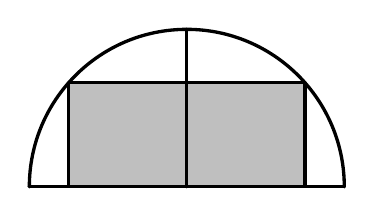
\begin{tikzpicture}[scale=1, line join=round, line cap=round, very thick]
			% Define parameters
			\def\R{2} % Radius of the semicircle
			\def\xrect{1.5} % Half-width of the rectangle
			
			% Calculate rectangle height using Pythagorean theorem
			\pgfmathsetmacro{\yrect}{sqrt(\R^2-\xrect^2)}
			
			% Define key coordinates
			\coordinate (L) at (-\R, 0);      % Left end of diameter
			\coordinate (RR) at (\R, 0);     % Right end of diameter (using RR to avoid conflict with \R)
			\coordinate (TC) at (0, \R);     % Top Center of semicircle arc
			\coordinate (BC) at (0, 0);     % Bottom Center (Origin)
			
			\coordinate (BL) at (-\xrect,0); % Bottom Left of rectangle
			\coordinate (BR) at (\xrect,0); % Bottom Right of rectangle
			\coordinate (TR) at (\xrect,\yrect); % Top Right of rectangle
			\coordinate (TL) at (-\xrect,\yrect); % Top Left of rectangle
			
			% Fill the rectangle first (so lines are drawn on top)
			\fill[gray!50] (BL) rectangle (TR);
			
			% Draw the semicircle arc
			\draw (L) arc (180:0:\R);
			
			% Draw the diameter
			\draw (L) -- (RR);
			
			% Draw the rectangle outline
			\draw (BL) rectangle (TR);
			
			% Draw the vertical line (axis of symmetry) passing through the rectangle
			\draw (BC) -- (TC);
			
		\end{tikzpicture}
	}
	\loigiai{
		\begin{center}
			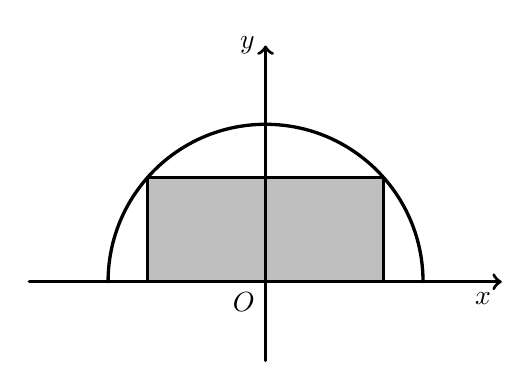
\begin{tikzpicture}[scale=1, line join=round, line cap=round, very thick]
				% Define parameters
				\def\R{2} % Radius of the semicircle
				\def\xrect{1.5} % Half-width of the rectangle
				
				% Calculate rectangle height using Pythagorean theorem
				\pgfmathsetmacro{\yrect}{sqrt(\R^2-\xrect^2)}
				
				% Define key coordinates
				\coordinate (L) at (-\R, 0);      % Left end of diameter
				\coordinate (RR) at (\R, 0);     % Right end of diameter (using RR to avoid conflict with \R)
				\coordinate (TC) at (0, \R);     % Top Center of semicircle arc
				\coordinate[label=below left:$O$] (BC) at (0, 0);     % Bottom Center (Origin)
				
				\coordinate (BL) at (-\xrect,0); % Bottom Left of rectangle
				\coordinate (BR) at (\xrect,0); % Bottom Right of rectangle
				\coordinate (TR) at (\xrect,\yrect); % Top Right of rectangle
				\coordinate (TL) at (-\xrect,\yrect); % Top Left of rectangle
				
				% Fill the rectangle first (so lines are drawn on top)
				\fill[gray!50] (BL) rectangle (TR);
				
				% Draw the semicircle arc
				\draw (L) arc (180:0:\R);
				
				% Draw the diameter
				\draw (L) -- (RR);
				
				% Draw the rectangle outline
				\draw (BL) rectangle (TR);
				
				% Draw the vertical line (axis of symmetry) passing through the rectangle
				\coordinate (A) at (-3,0);
				\coordinate[label=below left:$x$] (B) at (\R+1,0);
				\draw[->] (A)--(B);
				\coordinate[label=left:$y$] (C) at (0,\R+1);
				\coordinate (D) at (0,-1);
				\draw[->] (D)--(C);
			\end{tikzpicture}
		\end{center}
		Gọi $x$ là chiều dài của tấm giấy hình chữ nhật ($0<x<4$), $y$ là chiều rộng của tấm giấy hình chữ nhật ($0<y<2$).\\
		Ta có $\left(\dfrac{x}{2};y\right)$ là tọa độ của một đỉnh hình chữ nhật thuộc nửa đường tròn.\\
		Khi đó, ta được $$\dfrac{x^2}{4}+y^2=4\Leftrightarrow y^2=4-\dfrac{x^2}{4}=\dfrac{1}{4}(16-x^2)\Rightarrow y=\dfrac{1}{2}\sqrt{16-x^2}.$$
		Diện tích miếng giấy hình chữ nhật $S=xy=\dfrac{1}{2}x\sqrt{16-x^2}=\dfrac{1}{2}\sqrt{16x^2-x^4}$.\\
		Đặt $f(x)=16x^2-x^4$, có $f'(x)=32x-4x^3$. \\
		Xét $f'(x)=0 \Leftrightarrow \hoac{&x=2\sqrt{2}\\&x=-2\sqrt{2}.}$\\
		Ta có bảng biến thiên
		\begin{center}
			
\begin{tikzpicture}[>=stealth]
				\tkzTabInit[nocadre=false,lgt=1,espcl=2,deltacl=0.5]{$x$/.7 ,$f'(x)$/.7,$f(x)$/2}
				{$0$ , $2\sqrt{2}$ , $4$}
				\tkzTabLine{ ,+, $0$ ,-, }
				\tkzTabVar{-/$0$ , +/$64$ , -/$0$}
			\end{tikzpicture}
			
		\end{center}
		Vậy diện tích lớn nhất của miếng giấy hình chữ nhật là $\dfrac{1}{2}\sqrt{64}=4$.
	}
\end{ex}

\begin{ex}%[2D1V3-6]
	(\textit{Đề kiểm tra HK1 -- Trường THPT Ngô Gia Tự -- Năm 2024--2025})\\
	Từ một tấm bìa cứng hình vuông cạnh $ 30$ cm, người ta cắt bốn góc bốn hình vuông bằng nhau rồi gấp lại tạo thành hình hộp chữ nhật không nắp. Tìm cạnh hình vuông bị cắt để hình hộp chữ nhật tạo ra có thể tích lớn nhất.
	\begin{center}
		\begin{tikzpicture}[line join=round, line cap=round,>=stealth,font=\footnotesize,scale=0.8]
			\draw (0,0)--(4,0)--(4,4)--(0,4)--cycle;
			\draw[thin,pattern=north east lines] (0,0)--(1,0)--(1,1)--(0,1)--cycle (4,0)--(4,1)--(3,1)--(3,0)--cycle (4,3)--(4,4)--(3,4) node[midway,sloped,above]{$ x $}--(3,3)--cycle (0,4)--(0,3)--(1,3)--(1,4)--cycle;
			\draw[dashed] (1,1)--(3,1)--(3,3)--(1,3)--cycle;
			\draw[<->](-0.2,0)--(-0.2,4) node[midway,sloped,above]{$ 30\mathrm{~cm} $};
		\end{tikzpicture}
		\hspace{2cm}
		\begin{tikzpicture}[line join=round,line cap=round,line width=.6pt,font=\footnotesize,scale=1]
			\coordinate (B) at (0,0);
			\coordinate (A) at (1.5,1.8);
			\coordinate (C) at (4,0);
			\coordinate (D) at ($(C)-(B)+(A)$);
			\coordinate (H) at ($(B)!1/3!(D)$);
			\coordinate (A1) at ($(A)+(90:1)$);
			\coordinate (B1) at ($(B)-(A)+(A1)$);
			\coordinate (C1) at ($(C)-(A)+(A1)$);
			\coordinate (D1) at ($(D)-(A)+(A1)$);
			\draw (B1)--(B)--(C)--(D)--(D1)--(A1)--(B1)--(C1)--(D1) (C)--(C1);
			\draw[dashed] (A)--(D) (A1)--(A)--(B);
		\end{tikzpicture}
	\end{center}
	\loigiai{
		Gọi $ x $ là cạnh hình vuông bị cắt ($ 0\le x\le 15 $).\\
		Khi đó thể tích của khối hình chữ nhật tạo thành là 
		$$ V(x)=x\cdot \left(30-2x\right)^2= 4x^3-120x^2+900x.$$
		Suy ra $V'(x)=12 x^2-240 x+900$; $ V'(x)=0\Leftrightarrow \hoac{&x=5\\&x=15.} $\\
		Bảng biến thiên:
		\begin{center}
			
\begin{tikzpicture}
				\tkzTabInit[espcl=2.5,lgt=1.5]
				{$x$/0.7,$V'(x)$/0.7,$V(x)$/2.1}
				{$-\infty$,$5$,$15$}
				\tkzTabLine{,+,0,-,}
				\tkzTabVar{-/$-\infty$,+/$2\,000$,-/$0$}
			\end{tikzpicture}
		\end{center}
		Vậy thể tích khối hộp chữ nhật lớn nhất khi cạnh hình vuông bị cắt là $5$ cm.
	}
\end{ex}

\begin{ex}%[2D1V3-6]
	(\textit{Đề kiểm tra HK1 -- Trường THPT Nguyễn Thái Bình -- Năm 2024--2025})\\
	Doanh số bán hệ thống âm thanh mới đưa ra thị trường trong một khoảng thời gian dự kiến sẽ tuân theo đường cong logistic $R(x)=\dfrac{5\,000}{1+5\mathrm{e}^{-x}}$, $x \geq 0$, 
	trong đó thời gian $x$ tính bằng năm. Khi đó, đạo hàm $R'(x)$ sẽ biểu thị tốc độ bán hàng. Tốc độ bán hàng sẽ đạt tối đa vào năm thứ bao nhiêu (làm tròn đến chữ số hàng đơn vị)?
	\loigiai{Ta có
		$R'(x)= \dfrac{25\,000\mathrm{e}^{-x}}{\left(1+5\mathrm{e}^{-2}\right)^2}$, $x\geq 0$.\\
		Tốc độ bán hàng đạt tối đa khi $R'(x)$ đạt giá trị lớn nhất, ta cần tìm giá trị lớn nhất của $R'(x)$ trên $[0;+\infty)$.\\
		Ta có 
		\[
		R"(x)=-25\,000\cdot \dfrac{\mathrm{e}^{-x}\left(1+5\mathrm{e}^{-x}\right)^2+\mathrm{e}^{-x}\cdot 2\left(1+5\mathrm{e}^{-x}\right)\cdot5\mathrm{e}^{-x}}{\left(1+5\mathrm{e}^{-x}\right)^4}=\dfrac{25\,000\left(5\mathrm{e}^{-x}-1\right)}{\left(1+5\mathrm{e}^{-x}\right)^3.}
		\]
		Khi đó $R"(x)=0\Leftrightarrow 5\mathrm{e}^{-x}-1=0\Leftrightarrow x=\ln 5$.\\
		Bảng biến thiên
		\begin{center}
			
\begin{tikzpicture}[scale=1, line join=round, line cap=round, >=stealth]
				\tkzTabInit[nocadre, lgt=1.5, espcl=2.5, deltacl=0.5]
				{$x$/0.7, $R''(x)$/0.7, $R'(x)$/2}
				{$-\infty$,$\ln 5$, $+\infty$}
				\tkzTabLine{,+,0,-,}
				\tkzTabVar{-/, +/$1\,250$,-/$0$}
			\end{tikzpicture}	
		\end{center}
		Từ bảng biến thiên suy ra $R'$ đạt giá trị lớn nhất tại $x=\ln 5 \approx 1{,}61$. \\
		Vậy tốc độ bán hàng đạt tối đa vào thời điểm năm thứ hai.
	}
\end{ex}
\begin{ex}%[2D1V3-6]
	(\textit{Đề kiểm tra HK1 -- Trường THPT Thực hành Sư Phạm-- Năm 2024--2025})\\
	\immini{
		Một trang sách có dạng hình chữ nhật với diện tích là $384$ cm$^2$. Sau khi để lề trên và lề dưới đều là $3$ cm, để lề trái và lề phải đều là $2$ cm. Phần còn lại của trang sách được in chữ. Trang sách có kích thước tối ưu khi phần in chữ trên trang sách có diện tích lớn nhất. Tính chu vi của trang sách khi đạt kích thước tối ưu.
	}{
		\begin{tikzpicture}[>=stealth,smooth,line join=round,line cap=round,font=\footnotesize,scale=1]
			\path
			(0,0) coordinate (B)
			(0:3) coordinate (A)
			(90:4) coordinate (C)
			($(C)-(B)+(A)$) coordinate (D)
			;
			\fill[blue!20] (0.3,0.35) rectangle (2.7,3.65);
			\draw[dashed] (0.3,0.35) rectangle (2.7,3.65);
			;
			\draw (A)--(B)--(C)--(D)--(A)
			;
		\end{tikzpicture}
	}
	\loigiai{
		Gọi $x$ cm là chiều rộng của trang sách. Khi đó, chiều dài của trang sách là $\dfrac{384}{x}$ cm.\\
		Sau khi để lề thì phần in chữ có dạng hình chữ nhật có chiều rộng là $x-4$ cm và chiều dài là $\dfrac{384}{x}-6$ cm.\\
		Rõ ràng, $x$ phải thỏa mãn điều kiện $4<x<64$.\\
		Diện tích phần in chữ trên trang sách là
		\[S(x)=(x-4)\left(\dfrac{384}{x}-6\right)=\dfrac{-6x^2+408x-1\,536}{x}\,\left(\text{cm}^2\right)\]
		Xét hàm số $S(x)=\dfrac{-6 x^2+408 x-1\,536}{x}$ với $x \in(4;64)$.\\
		Ta có $S'(x)=\dfrac{-6 x^2+1\,536}{x^2}$;
		$S'(x)=0 \Rightarrow-6x^2+1\,536=0 \Leftrightarrow \hoac{&x=-16\\&x=16.}$\\
		Khi đó trên khoảng $(4; 64)$, $S'(x)=0$ khi $x=16$.\\
		Bảng biến thiên của hàm số $S(x)$ như sau
		\begin{center}
			
\begin{tikzpicture}[>=stealth,line join=round,line cap=round,font=\normalsize,scale=1]
				\tkzTabInit[nocadre,lgt=1.4,espcl=2.2,deltacl=0.5]{$x$/.7 ,$S'(x)$/.7,$S(x)$/2}
				{$4$ , $16$ , $64$}
				\tkzTabLine{ ,+, $0$ ,-, }
				\tkzTabVar{-/$0$ , +/$216$ , -/$0$}
			\end{tikzpicture}
		\end{center}
		Dựa vào bảng biến thiên, ta thấy trên khoảng $(4;64)$, hàm số $S(x)$ đạt giá trị lớn nhất bằng $216$ tại $x=16$.\\
		Khi đó, chiều dài của trang sách là $\dfrac{384}{16}=24$.\\
		Do đó chu vi của trang sách là $2\cdot(16+24)=80$ cm.
	}
\end{ex}
\begin{ex}%[2D1V3-6]
	(\textit{Đề kiểm tra HK1 -- Trường THPT Thực hành Sư Phạm -- Năm 2024--2025}) \\
	Một nhà máy dự định sản xuất không quá $900$ sản phẩm. Nếu nhà máy sản xuất $x$ sản phẩm $(0\leq x \leq 900)$ thì lợi nhuận nhận được khi bán hết số sản phẩm đó là
	\[f(x)=-x^3+900 x^2+56\,700 x+450\,000\, \text{(đồng).}\]
	Nhà máy cần sản xuất bao nhiêu sản phẩm để lợi nhuận thu được là lớn nhất?
	\loigiai{
		Hàm lợi nhuận khi bán hết $x$ sản phẩm là 
		$$f(x)=-x^3+900 x^2+56\,700 x+450\,000,\,(0 \leq x \leq 900).$$
		Ta có $f'(x)=-3x^2+1\,800 x+56\,700$.\\
		$f'(x)=0 \Leftrightarrow\hoac{&x=630 \in[0;900] \\&x=-30 \notin[0;900].}$\\	
		Ta có $f(0)=450\,000$; $f(630)=143\,334\,000$; $f(900)=51\,480\,000$.\\
		Vậy lợi nhuận thu được lớn nhất bằng $f(630)=143\,334\,000$ khi nhà máy sản xuất $630$ sản phẩm.
	}
\end{ex}
\begin{ex}%[2D1V3-6]
	(\textit{Đề kiểm tra HK1 -- Trường THPT Quế Sơn -- Năm 2024--2025}) \\
	Một hộ làm nghề dệt vải lụa tơ tằm sản xuất mỗi ngày được $x$ mét vải lụa ($1 \le x \le 20$). Tổng chi phí sản xuất $x$ mét vải lụa (nghìn đồng) cho bởi hàm chi phí $C(x)=2x^3-30x^2-126x+2\,222$.
	Giả sử hộ làm nghề dệt này bán hết sản phẩm dệt ra mỗi ngày với giá $210$ nghìn đồng/mét. Hãy tính lợi nhuận tối đa (nghìn đồng) của hộ này trong một ngày.
	
%	\par	\shortans{2874}
	\loigiai{
		Hàm doanh thu mỗi ngày là $R(x)=210x $ (nghìn đồng).\\
		Hàm lợi nhuận mỗi ngày là:\\ 
		$L(x)=R(x)-C(x)=210x-(2x^3-30x^2-126x+2\,222)=-2x^3+30x^2+336x-2\,222,\forall x \in [1;20]$.\\
		Ta có $	L'(x)=-6x^2+60x+336,\forall x \in [1;20]$. \\
		Ta có $ L'(x)=0  \Leftrightarrow 	-6x^2+60x+336=0 \Leftrightarrow x^2-10x-56=0 \Leftrightarrow \hoac{
			&x=14 \\
			&x=-4 \ (\text{loại}).}$\\
		Ta có $L(1)=-1\,858$, $L(14)=2\,874$, $L(20)=498$.\\
		Vậy lợi nhuận tối đa là $2\,874$ nghìn đồng.
	}
	
\end{ex}
\begin{ex}%[2D1V3-6]
	(\textit{Đề kiểm tra HK1 -- Trường THPT Lý Thường Kiệt -- Năm 2024--2025}) \\
	Từ một miếng bạt hình vuông cạnh $18$ m như hình vẽ dưới đây. Người ta dự tính cắt đi phần tô đậm của tấm bạt rồi gập và may lại (các đường may không đáng kể) để phủ lên tháp trang trí (có dạng hình chóp tứ giác đều) để tránh hư hại khi trời mưa. Biết khối chóp hình thành sau khi gập và may lại cần thể tích lớn nhất thì mới phủ kín tháp đèn. Hỏi thể tích khối chóp đạt giá trị lớn nhất bằng bao nhiêu mét khối? (kết quả làm tròn tới hàng đơn vị).
	\begin{center}
		\begin{tikzpicture}[>=stealth,line join=round,line cap=round,font=\footnotesize,scale=1]
			\tikzset{declare function={a=4;b=.3;}}
			\path 
			(0,0)coordinate (A)++(0:a)coordinate (B)++(-90:a)coordinate (C)++(180:a)coordinate (D)
			($($(A)!.5!(B)$)!b!{90}:(A)$)coordinate (E)
			($($(C)!.5!(B)$)!b!{90}:(B)$)coordinate (F)
			($($(C)!.5!(D)$)!b!{90}:(C)$)coordinate (G)
			($($(A)!.5!(D)$)!b!{90}:(D)$)coordinate (H)
			;	
			\foreach \po/\pt/\ptt in{A/E/B,B/F/C,C/G/D,D/H/A} {
				\fill[gray!30] (\po)--(\pt)--(\ptt)--cycle;
			}
			\foreach \pointo/\pointt in {A/B,B/C,C/D,D/A,A/E,E/F,F/G,G/H,H/E,B/E,B/F,C/F,C/G,D/G,A/H,D/H}{
				\draw[fill=black](\pointo)--(\pointt);
			}
		\end{tikzpicture}\quad\qquad
		\begin{tikzpicture}[>=stealth,line join=round,line cap=round,font=\footnotesize,scale=1]
			\tikzset{
				pics/hinhChopTuGiacDeu/.style  n args={6}{
					code={
						\tikzset{
							declare function={a=3;b=1.5;h=3;goc=-140;}
						}	
						\path 
						(0,0)coordinate (#1)+(0:a)coordinate (#2)+(goc:b)coordinate (#4)			
						($(#2)+(#4)-(#1)$)coordinate (#3)
						(intersection of #1--#3 and #2--#4)coordinate (#5) ($(#5)+(90:h)$)coordinate (#6)
						;
					}
			}}
			\path 
			(0,0)pic {hinhChopTuGiacDeu={A}{B}{C}{D}{O}{S}}
			;	
			\foreach \pointo/\pointt in {A/D,A/B,S/A}{
				\draw[fill=black,dashed](\pointo)--(\pointt);
			}	
			\foreach \pointo/\pointt in {S/C,S/B,S/D,B/C,C/D}{
				\draw[fill=black](\pointo)--(\pointt);
			}
		\end{tikzpicture}
	\end{center}		
%	\shortans{197}
	\loigiai{
		\begin{center}
			\begin{tikzpicture}[>=stealth,line join=round,line cap=round,font=\footnotesize,scale=1]
				\tikzset{declare function={a=4;b=.3;}}
				\path 
				(0,0)coordinate (A)++(0:a)coordinate (B)++(-90:a)coordinate (C)++(180:a)coordinate (D)
				($($(A)!.5!(B)$)!b!{90}:(A)$)coordinate (E)
				($($(C)!.5!(B)$)!b!{90}:(B)$)coordinate (F)
				($($(C)!.5!(D)$)!b!{90}:(C)$)coordinate (G)
				($($(A)!.5!(D)$)!b!{90}:(D)$)coordinate (H)
				($(A)!.5!(B)$)coordinate (I)
				($(D)!.5!(C)$)coordinate (J)
				;	
				\foreach \po/\pt/\ptt in{A/E/B,B/F/C,C/G/D,D/H/A} {
					\fill[gray!30] (\po)--(\pt)--(\ptt)--cycle;
				}
				\foreach \pointo/\pointt in {A/B,B/C,C/D,D/A,A/E,E/F,F/G,G/H,H/E,B/E,B/F,C/F,C/G,D/G,A/H,D/H,I/J}{
					\draw[fill=black](\pointo)--(\pointt);
				}
				\foreach \point/\goc in {A/130,B/70,C/-60,D/210,I/90,J/-90,E/50,F/0,G/-60,H/180}{
					\draw[fill=black](\point)circle(.8pt)+(\goc:2mm)node[scale=.8]{$\point$};
				}
			\end{tikzpicture}\quad\qquad
			\begin{tikzpicture}[>=stealth,line join=round,line cap=round,font=\footnotesize,scale=1]
				\tikzset{
					pics/hinhChopTuGiacDeu/.style  n args={6}{
						code={
							\tikzset{
								declare function={a=3;b=1.5;h=3;goc=-140;}
							}	
							\path 
							(0,0)coordinate (#1)+(0:a)coordinate (#2)+(goc:b)coordinate (#4)			
							($(#2)+(#4)-(#1)$)coordinate (#3)
							(intersection of #1--#3 and #2--#4)coordinate (#5) ($(#5)+(90:h)$)coordinate (#6)
							;
						}
				}}
				\path 
				(0,0)pic {hinhChopTuGiacDeu={E}{F}{G}{H}{O}{S}}
				;	
				\foreach \pointo/\pointt in {E/F,E/H,S/E,E/G,F/H,S/O}{
					\draw[fill=black,dashed](\pointo)--(\pointt);
				}	
				\foreach \pointo/\pointt in {S/G,S/F,S/H,F/G,G/H}{
					\draw[fill=black](\pointo)--(\pointt);
				}
				\foreach \point/\goc in {S/90,E/150,F/-10,G/-60,H/210,O/-90}{
					\draw[fill=black](\point)circle(.8pt)+(\goc:2mm)node[scale=.8]{$\point$};
				}
			\end{tikzpicture}
		\end{center}	
		Ký hiệu như hình vẽ trên.\\
		Với $I$, $J$ lần lượt là trung điểm của  $AB$ và $CD$.\\
		Gọi $O$ là giao điểm của $EG$ và $FH$.\\
		Ta có $AI=IB=\dfrac{1}{2} AB=9$.\\
		Đặt $EF=FG=GH=HE=x$,  $\left(0 < x < 9\sqrt{2}\right)$.\\
		Khi đó $\heva{&EG=FH=x\sqrt{2}\\&EI=GJ=\dfrac{18-x\sqrt{2}}{2}.}$\\
		Suy ra $EI=GJ=\dfrac{18-2\sqrt{x}}{2}$.\\
		Do đó 
		\[
		AE=\sqrt{AI^2+IE^2}=\sqrt{9^2+\left( \dfrac{18-x\sqrt{2}}{2} \right)^2}=\sqrt{\dfrac{x^2}{2}-9\sqrt{2}x+162}.
		\]
		Ta có $SE=AE=\sqrt{\dfrac{x^2}{2}-9\sqrt{2}x+162}$.\\
		Suy ra
		\[
		SO=\sqrt{SE^2-OE^2}=\sqrt{\dfrac{x^2}{2}-9\sqrt{2}x+162-\dfrac{x^2}{2}}=\sqrt{162-9\sqrt{2}x}.
		\]
		Thể tích khối chóp là
		\[
		V=\dfrac{1}{3} \cdot SO \cdot S_{EFGH}=\dfrac{1}{3} \cdot \sqrt{162-9\sqrt{2}x} \cdot x^2.
		\]
		Khi đó $V'(x)=\left(\dfrac{1}{3} \cdot \sqrt{162-9\sqrt{2}x} \cdot x^2\right)'=\dfrac{-15\sqrt{2}x^2+216x}{2\sqrt{162-9\sqrt{2}x}}$.\\
		$V'(x)=0\Rightarrow x= \dfrac{36\sqrt{2}}{5}$.\\
		Ta có bảng biến thiên
		\begin{center}
			
\begin{tikzpicture}[>=stealth,line join=round,line cap=round,font=\footnotesize,scale=1]
				\tkzTabInit[nocadre=true,lgt=1.2,espcl=3,deltacl=.55]
				{$x$/0.8, $V'(x)$/0.7, $V(x)$/1.8}
				{$0$,$\dfrac{36\sqrt{2}}{5}$,$9\sqrt{2}$}
				\tkzTabLine{,+,$0$,-,}
				\tkzTabVar{-/,+/$197$,-/}	
			\end{tikzpicture}			
		\end{center}
		Từ bảng biến thiên cho thấy thể tích của khối chóp đạt giá trị lớn nhất là $197$ khi $x=\dfrac{36\sqrt{2}}{5}$ m.
	}
\end{ex}
\Closesolutionfile{ans}